% CVPR 2024 Paper Template; see https://github.com/cvpr-org/author-kit

\documentclass[10pt,twocolumn,letterpaper]{article}

%%%%%%%%% PAPER TYPE  - PLEASE UPDATE FOR FINAL VERSION
\usepackage{cvpr}              % To produce the CAMERA-READY version
% \usepackage[review]{cvpr}      % To produce the REVIEW version
% \usepackage[pagenumbers]{cvpr} % To force page numbers, e.g. for an arXiv version

% Import additional packages in the preamble file, before hyperref
%
% --- inline annotations
%
\newcommand{\red}[1]{{\color{red}#1}}
\newcommand{\todo}[1]{{\color{red}#1}}
\newcommand{\TODO}[1]{\textbf{\color{red}[TODO: #1]}}
% --- disable by uncommenting  
% \renewcommand{\TODO}[1]{}
% \renewcommand{\todo}[1]{#1}
\usepackage{amsthm}
\usepackage{graphicx}
\usepackage{animate}
\newcommand{\Var}{\textup{Var}}
\newcommand{\Cov}{\textup{Cov}}
\newcommand{\bE}{\mathbb{E}}
\newtheorem{proposition}{Proposition}
\newtheorem{example}{Example}


% It is strongly recommended to use hyperref, especially for the review version.
% hyperref with option pagebackref eases the reviewers' job.
% Please disable hyperref *only* if you encounter grave issues, 
% e.g. with the file validation for the camera-ready version.
%
% If you comment hyperref and then uncomment it, you should delete *.aux before re-running LaTeX.
% (Or just hit 'q' on the first LaTeX run, let it finish, and you should be clear).
\definecolor{cvprblue}{rgb}{0.21,0.49,0.74}
\usepackage[pagebackref,breaklinks,colorlinks,citecolor=cvprblue]{hyperref}
\usepackage{comment,amsmath}

%%%%%%%%% PAPER ID  - PLEASE UPDATE
\def\paperID{14662} % *** Enter the Paper ID here
\def\confName{CVPR}

\def\confYear{2024}

\newcommand{\bp}[1]{\textcolor{red}{{[#1]}}}

%%%%%%%%% TITLE - PLEASE UPDATE


\title{MAGICK: A Large-scale Captioned Dataset from Matting Generated Images using Chroma Keying }
\newcommand{\methodname}{MAGICK}

%%%%%%%%% AUTHORS - PLEASE UPDATE
\author{Ryan D. Burgert\hspace{-10mm}\\
Stony Brook University\\
{\tt\small rburgert@cs.stonybrook.edu}
\and
Brian L. Price\hspace{-10mm}\\
Adobe Research\\
{\tt\small bprice@adobe.com}
\and
Jason Kuen\hspace{-10mm}\\
Adobe Research\\
{\tt\small jkuen@adobe.com}
\and
Yijun Li\hspace{-10mm}\\
Adobe Research\\
{\tt\small yijli@adobe.com}
\and
Michael S. Ryoo\\
Stony Brook University\\
{\tt\small mryoo@cs.stonybrook.edu}
}




\begin{document}
\maketitle
\begin{abstract}

Generative modeling aims to transform random noise into structured outputs. In this work, we enhance video diffusion models by allowing motion control via structured latent noise sampling. This is achieved by just a change in data: we pre-process training videos to yield structured noise. Consequently, our method is agnostic to diffusion model design, requiring no changes to model architectures or training pipelines. Specifically, we propose a novel noise warping algorithm, fast enough to run in real time, that replaces random temporal Gaussianity with correlated warped noise derived from optical flow fields, while preserving the spatial Gaussianity. The efficiency of our algorithm enables us to fine-tune modern video diffusion base models using warped noise with minimal overhead, and provide a one-stop solution for a wide range of user-friendly motion control: local object motion control, global camera movement control, and motion transfer. The harmonization between temporal coherence and spatial Gaussianity in our warped noise leads to effective motion control while maintaining per-frame pixel quality. Extensive experiments and user studies demonstrate the advantages of our method, making it a robust and scalable approach for controlling motion in video diffusion models. Video results are available on our \href{https://eyeline-research.github.io/Go-with-the-Flow/}{webpage}; source code and model checkpoints are available on \href{https://github.com/Eyeline-Research/Go-with-the-Flow}{GitHub}.

\end{abstract}    
\vspace{-5mm}
\section{Introduction}
\label{locVLM_sec:intro}

Holistic visual understanding requires learning beyond simply content of an image to encompass awareness on spatial locations of objects and their relations \cite{marr1982vision}. In the context of visual question answering (VQA), such spatial awareness allows better reasoning involving structural and contextual information contained within an image \cite{chen2023shikra}.

Since the introduction of powerful large-language models (LLMs) such as GPT-3 \cite{brown2020language}, Chat-GPT \cite{gpt4}, Vicuna \cite{vicuna2023}, and LLaMA~\citep{touvron2023llama,touvron2023llama2} that are capable of human style conversation, their visual counterparts such as BLIP-2 \cite{li2023blip}, LLaVA \cite{liu2023visual} have enabled novel tasks within the vision modality. However, despite their \cite{li2023blip,liu2023visual} highly generic visual understanding, these models exhibit poor language-based spatial reasoning \cite{chen2023shikra}. In fact, they fail at simple tasks such as distinguishing whether an object lies to the left or right of another object (see \cref{locvlm_tbl:spatial_icl}). 
% half of the image

\begin{figure}[t]
\centering

\includegraphics[width=.5\linewidth]{figures__intro1.png}\\
\texttt{man with blonde hair in blue shirt and brown pants}

\includegraphics[width=.5\linewidth]{figures__intro2.png}\\
\texttt{bald man wearing glasses with white shirt and black pants}

\caption{\textbf{Zero-Shot Segmentation with phrases}:  We highlight the ability of \modelname to ground complex language prompts onto an image with no segmentation specific training. An off-the-shelf diffusion model is used with only an inference time optimization technique to generate these segmentations. If you look closely, you'll notice the bald man's arms are segmented - but are not visible in the photo! Peekaboo has fairly strong shape priors.}
\label{fig:intro}
\end{figure}


In the case of contrastive language image models (such as CLIP \cite{radford2021learning}, ALIGN \cite{Jia2021ScalingUV}), recent works explore how injecting explicit spatial awareness \cite{Zhang2023AssociatingSG,Luo2022SegCLIPPA,Mukhoti2022OpenVS,Ranasinghe2022PerceptualGI} can enable more holistic visual understanding. In fact, \cite{Ranasinghe2022PerceptualGI} shows how such improved spatial awareness benefits model robustness in adversarial domains. 
This raises the question of how generative language image models, particularly those connecting LLMs to visual encoders \cite{li2023blip,liu2023visual} can benefit from such spatial awareness specific training. We refer to models of this category that generate textual outputs given joint image-text inputs (e.g. \cite{li2023blip,liu2023visual}) as visual-LLMs (V-LLMs). 

In this work, we explore location specific instruction fine-tuning objectives that explicitly enforce V-LLMs to meaningfully process and generate textual image-space coordinates. We hypothesize that such training would lead to improved spatial awareness in these V-LLMs, therein improving performance on VQA tasks. To this end, we propose three instruction fine-tuning objectives that unify location representation with natural language. We also explore optimal representation forms for image-space locations and how pseudo-data generation can be leveraged for efficient scaling of our framework. We name our resulting model as LocVLM.  

While the idea of adapting V-LLMs to perform localization related tasks (e.g. detection, segmentation) using V-LLMs has been explored in multiple recent works \cite{zhang2023gpt4roi,zhao2023bubogpt,zang2023contextual,peng2023kosmos,You2023FerretRA,wang2023visionllm,lai2023lisa}, these approaches depend on task specific architectural modifications or treat localization inputs / outputs differently from natural language. In contrast, our LocVLM focuses on a unified framework treating location and language as a single modality of inputs with the goal of complementing performance in each task. We intuit that processing location represented in textual form would enforce the LLM to select appropriate image regions as opposed to relying on region level features provided by the architecture. At the same time, textual form location outputs promote spatial awareness at language level in a human interpretable manner, in contrast to using secondary heads or specialized tokens for location prediction.  
Concurrent work in \cite{chen2023shikra} also explores textual location representation with a generic V-LLM architecture similar to our work. Our proposed LocVLM differs with focus on optimal location representation forms, data-efficient pseudo-labelling, and video domain operation. 

Our proposed framework exhibits improved spatial awareness in VQA style conversation demonstrated through experimentation on 14 datasets across 5 vision-language tasks: Spatial Reasoning, Image VQA, Video VQA, Object Hallucination, and Region Description. 
We summarize our key contributions as follows: 
\begin{itemize}[leftmargin=2em,noitemsep,topsep=0.0ex,itemsep=-1.0ex,partopsep=0ex,parsep=1ex]
    \item Inject textual spatial coordinate awareness into V-LLMs 
    \item Propose three novel localization based instruction fine-tuning objectives for V-LLMs 
    \item Discover optimal coordinate representation forms 
    \item Pseudo-Data generation for improved region description and scaling to video domain
\end{itemize} 

\section{Related Work}
\label{sec:relatedwork}

\paragraph{Synthetic segmentation data generation:} 
Many methods have recently been proposed to synthetically generate segmentation data. Early methods utilize GANs for data synthesis.
DatasetGAN~\cite{zhang2021datasetgan} proposes to decode GAN latent codes to generate segmentation data, primarily of specifc object parts or of limited scenes like bedrooms.
BigDatasetGAN~\cite{zhang2022bigdatasetgan} produces masks for single primary objects by training a GAN on Imagenet~\cite{ILSVRC15}.

Diffusion-based model typically take a text prompt as input, then simultaneously synthesize an image along with a mask. The mask may be of a single primary object~\cite{wu2023diffumask,li2023open} or a semantic segmentation within the domain of an existing hand-labeled dataset~\cite{wu2023datasetdm,nguyen2023dataset}. Variations of this theme include generating multiple images and object masks at once~\cite{xie2023mosaicfusion} or generating the masks first and then the image~\cite{ye2023seggen}. Peekaboo~\cite{burgert2023peekaboo} generates single objects, the most closely related method to our own, but the results lack details like hair and fur. While arguments can be made against training with generated data~\cite{alemohammad2023selfconsuming,shumailov2023curse}, these works show that training with synthetic data, either alone or in conjunction with real data, yields results that are on par with or surpass the state-of-the-art set by methods trained with real data. 

A drawback of these methods is they all focus on binary masks and lack transparencies and fine details such as hair or fur. Our method specifically targets generating images with alpha mattes that exhibit fine details.



\vspace{-4mm}
\paragraph{Alpha matting datasets:}  
While our method is the first to generate images with alpha masks, many alpha matting datasets already exist. Generating alpha mattes is a difficult task, requiring complicated image capture methods and/or excessive user interaction, resulting in the existing matting datasets being small in size. The early matting dataset from alphamatting.com~\cite{rhemann2009perceptually} was generated using triangulation matting, a tedious process of photographing the same object against multiple backgrounds, resulting in a dataset of 27 training images and 8 test images. This was extended to video to produce a small number of frames using stop-motion photography~\cite{erofeev2015perceptually}. 

Manual extraction of the alpha matte from photographs using existing matting methods has been used to create several datasets~\cite{xu2017deep,shen2016deep,wang2021crgnn,sun2021semantic}. However, this approach is very time consuming and prone to error, generally resulting in only a few hundred objects.

Video matting datasets often use chroma keying~\cite{smith1996blue} to generate alpha data~\cite{zhang2021attention,lin2021real}. However, high quality chroma keying requires both careful setup of the green (blue) screen and lighting as well as manual post-processing to tweak parameters and manually correct or mask out mistakes.

While these methods can produce high-quality alpha mattes, they are difficult and tedious to collect. This contrasts our approach that can produce large numbers of accurate alpha mattes with the corresponding images with minimal user interaction.

\vspace{-4mm}
\paragraph{Segmentation and Matting:}  

Arguably, an alternative method of producing a dataset like ours would be to simply extract objects from generated images with standard segmentation/matting methods without bothering to produce them on green screens. Such generated images would contain background details and potentially other foreground objects that would need to be separated from the object.

While many segmentation datasets exist~\cite{lin2014microsoft,zhou2017scene,OpenImages,Cordts2016Cityscapes}, as do many methods for segmenting salient objects~\cite{li2014secrets,li2017instance,qin2022highly} or multiple objects~\cite{kirillov2019panoptic,he2018mask,Qi_2023_ICCV} from images, these methods would not yield the accurate alpha mattes that our method produces.  Matting methods~\cite{xu2017deep,soumyadip2020background,cai2019disentangled,lu2019indices,tang2019learning,dai2022boosting}, despite significant progress recently, are still imperfect and would include errors or artifacts in the alpha mattes. Indeed, we hope our dataset will be used to improve matting methods in future works.


\begin{comment}

\bp{Please cite segementatin methods such as dichotomous image segmentation for foreground selection and the photoshop subject selection if it exists. Also bring up the fact that there are many large sregmentation datasets, but these do not handle matting and are naturally imprecise even for segmentation (coco for example has fairly polygonal boundaries a lot of the time, and doesn't focus on single-subjects like ours does). (barring perhaps the https://xuebinqin.github.io/dis/index.html dichotomous image segmentation dataset, which contains under 6000 samples, all of which had to be manually annotated in gimp and *still* don't contain any matting information. }

\bp{
Important work to talk about because reviewers might try to poke a hole in this dataset because its synthetic:
%
Please also cite "The Curse of Recursion: Training on Generated Data Makes Models Forget" https://arxiv.org/abs/2305.17493 which talks about training on synthetic data. It cautions against it. Brifly mention that paper as it only focuses on LLM's. 
%
Another paper discussed this as well but in the context of image generation:
https://arxiv.org/pdf/2307.01850.pdf
%
They also mention that human-in-the-loop selection can mitigate the degredation of the models, albeit at the cost of sample diversity. However, as we're trying to make isolated subjects, this is arguable desirable. Empiricaly we show its usefulness, and they also mention that adding even a small amount of fresh data is enough to hold back this problem. 
%
I would also mention that this degradation takes more than 2 generations to become a large problem as indicated by the graphs in their paper, and we could always mix our dataset with some other datasets such as dichotomous image segmentation to boost it. 
%
From their paper: """Sampling bias plays a key rôle in autophagous loops. Users of generative models tend to manually curate (“cherry-pick”) their synthetic data, preferring high-quality samples and rejecting low-quality ones. Moreover, state-of-the-art generative models typically feature controllable parameters that can increase synthetic quality at the expense of diversity [42, 58]. We demonstrate that the sampling biases induced through such quality-diversity (precision-recall) trade-offs have a major impact on the behavior of an autophagous training loop. Specifically, we show that, without sampling bias, autophagy can lead to a rapid decline of both quality and diversity, whereas, with sampling bias, quality can be maintained but diversity degrades even more rapidly."""
%
}

\bp{Please also cite SDEDIT - I'm referencing that later in the paper, and show that colloquially its called im2im by both huggingface and the community (you can see that here - in a link in the comment of the code next to this text) 
% https://huggingface.co/docs/diffusers/api/pipelines/stable_diffusion/img2img 
so I'm calling it img2img as well}

\bp{Not in the related works, but we also have to cite: MSSSIM (multiscale structural image similarity) which is used in the similarity score metric for automatic selection, ControlNet. Canny edges controlnet is straightforward to explain but we also need to briefly explain what "scribbles" controlnet is (see the url in the comment below
%See https://huggingface.co/lllyasviel/sd-controlnet-scribble  --- they explain how they got their dataset. TLDR - it's based on HED edge detection
It's based on HED edge detection (https://arxiv.org/abs/1504.06375 - "Holistically-Nested Edge Detection"
}

\end{comment}
\section{Method}
\label{sec:method}

\method is comprised of two separate parts: our noise warping algorithm and video diffusion fine-tuning. The noise warping algorithm operates independently from the diffusion model training process: we use the noise patterns it produces to train the diffusion model. Our motion control is based \textit{entirely} on noise initializations, introducing no extra parameters to the video diffusion model.

Inspired by the existing noise warping algorithm HIWYN~\cite{chang2024warped}, which introduced noise warping for image diffusion models, we introduce a new use case for the warped noise: we use it as a form of \textit{motion conditioning} for video generation models. After fine-tuning a video diffusion model on a large corpus of videos paired with warped noise, we can control the motion of videos at inference time.

\subsection{\method noise warping}

% algorithm placeholder
\begin{algorithm}[t]
\caption{\method next-frame warping}
\label{alg:main}
\begin{algorithmic}[1]
\State \textbf{Input:} previous-frame noise $q \in \mathbb{R}^{D}$, previous-frame density $p \in \mathbb{R}^{D}$, forward flow $f: D \to \mathbb{N}^2$, backward flow $f': D \to \mathbb{N}^2$.
\State Let $G = (V, V', E)$ be a bipartite graph with $V = D$, $V' = D$ and edge set $E = \{\}$ to be constructed. % this is really unecessary: \Comment{$E$ only contains edges from $V$ to $V'$.}
\For{$v$ in $V$} \Comment{Contraction}
\State $E \gets E \cup (v, v+f(v))$ if $v+f(v')\in D$
\EndFor
\For{$v'$ in $V'$} \Comment{Expansion}
\If{$\deg_G(v') = 0$} \Comment{$\deg_G(v)$ denote the degree of $v$ in $G$}
\State $E \gets E \cup (v' + f'(v'), v')$ if $v' + f'(v')\in D$
\EndIf
\EndFor
\For{$v$ in $V$} \Comment{Conditional white noise sampling}
\State $d \gets \deg_G(v)$
\State Sample $Z \sim \mathcal{N}(0, I_{d})$, and set $S \gets \sum_{i=1}^d Z_i$
\State $X_i \gets \frac{q(v)}{d} + \frac{1}{\sqrt{d}}(Z_i - \frac{S}{d})$ for $i \in [d]$
\State $R(v) \gets \{X_i\}_{i\in[d]}$ 
\EndFor
\For{$(v')$ in $V'$} \Comment{Compute next-frame noise and density}
\State $q'(v') \gets 0$, $p'(v') \gets 0$, $s \gets 0$
\For{{$v$ in $V$ such that $(v,v') \in E$}}
\State $d \gets \deg_G(v)$, $\alpha \gets \frac{p(v)}{d}$
\State $q'(v') \gets q'(v') + \alpha R(v)\text{.pop}()$
\State $p'(v') \gets p'(v') + \alpha$
\State $s \gets s + \alpha^2 \frac{1}{d}$
\EndFor
\If{$s = 0$}
\State Sample $q'(v') \sim \mathcal{N}(0, 1)$
\Else
\State $q'(v') \gets \frac{q'(v')}{\sqrt{s}}$ \Comment{Renormalize to unit variance}
\EndIf
\EndFor
\State \textbf{return} next-frame noise and density $q', p'$.
\end{algorithmic}
\label{alg:algorithm}
\end{algorithm}


\subsubsection{Algorithm}


To facilitate the large-scale noise warping required by this new use case, we introduce a fast noise warping algorithm (\cref{alg:main}) that warps noise frame-by-frame, storing just the previous frame's noise (with dimensions $H \times W \times C$, where $H$ is height, $W$ is width, and $C$ is the number of channels) and a matrix of per-pixel flow density values (with dimensions $H \times W$). The density values indicate how much noise has been compressed into a given region. Unlike HIWYN~\cite{chang2024warped} which requires time-consuming polygon rasterization and upsampling of each pixel, our algorithm directly tracks the necessary \textit{expansion} and \textit{contraction} between frames according to the optical flow and uses only pixel-level operations that are easily parallelizable. We show that our algorithm retains the same Gaussianity guarantee as HIWYN~\cite{chang2024warped} (\cref{prop:gaussianity}).

\noindent \textbf{Next-frame noise warping}. Our noise warping algorithm calculates noise iteratively, where the noise for a given frame depends only on the state of the previous frame.

Let $H\times W$ be the dimensions of each video frame. Let $D = [H]\times [W]$ denote a 2D matrix with height $H$ and width $W$, where we use the notation $[n]:= {1,\ldots, n}$. Given the previous frame's noise\footnote{Since different channels are treated independently, we will assume a single channel in images.} $q \in \mathbb{R}^D$ and the flow density $p \in \mathbb{R}^D$ together with forward and backward flows\footnote{We allow flows to go out of bounds, i.e., $f$ and $f'$ can land in $\mathbb{N}^2 \setminus D$.} $f,f':D\to \mathbb{N}^2$, our algorithm computes the next-frame noise and density $q',p' \in \mathbb{R}^D$ such that $q'$ (resp. $p'$) is temporally correlated with $q$ (resp. $p$) via the flows.

At a high level, our algorithm (in~\cref{alg:algorithm}) combines two types of dynamics: \textit{expansion} and \textit{contraction}. In the case of \textit{expansion}, such as when a region of the video zooms in or an object moves towards the camera, one noise pixel is mapped to one or more noise pixels in the next frame (hence it ``expands''). In the case of \textit{contraction}, we adopt the Lagrangian fluid dynamics viewpoint of treating noise pixels as particles moving along the forward flow $f$. This often leaves gaps that need to be filled. Hence, for regions not reached when flowing along $f$, we use the backward flow $f'$ to pull back a noise pixel. That gap is filled with noise calculated with the \textit{expansion} case.

Additionally, to preserve the distribution correctly over long time periods, we use density values to keep track of how many noise pixels were aggregated into a given region, so that when mixed with other nearby particles in the \textit{contraction} case, these higher density particles have a larger weight. This is illustrated in \cref{fig:algorithm_diagram}.

We unify both \textit{expansion} and \textit{contraction} cases by building a bipartite graph $G$ where edges represent how noise and density should be transferred from the previous frame to the next. When aggregating the influence from graph edges to form the next-frame noise $q'$, we scale the noise in accordance with the flow density to ensure the preservation of the original frame's distribution, as detailed in ~\cref{alg:algorithm}. The \textit{expansion} and \textit{contraction} cases are calculated in tandem to prevent any cross-correlation, guaranteeing the output will be perfectly Gaussian.


\subsubsection{Theoretical analysis}

\begin{figure}
    \centering
    \includegraphics[width=\linewidth]
    {fig/algo_diagram_2_layers.png}
    \caption{Diagram of our noise warping algorithm. A case example of our algorithm illustrates both the \textit{expansion} and \textit{contraction} cases, along with example density values. Each node represents some noise pixel `q'. Noise values $q_{0..3}$ are transferred from frame 0 to frame 1 using forward optical flow, and the remaining pixels in frame 1 that did not receive any values obtain their values from frame 0 using reverse optical flow (the \textit{expansion} case). In the \textit{contraction} cases such as $q'_2$, their densities become the sum of their sources. And in the \textit{expansion} case, where one source pixel spreads out into multiple target pixels, such as $q_2$ spreading out into $q'_1$ and $q'_3$, its density is dispersed.}
    \label{fig:algorithm_diagram}
\end{figure}

\begin{proposition}[Preservation of Gaussian white noise]
\label{prop:gaussianity}
If the pixels of the previous-frame noise $q$ in \cref{alg:main} are i.i.d. standard Gaussians, then the output next-frame noise $q'$ also has i.i.d. standard Gaussian pixels. Please check the appendix for a formal mathematical proof.
\end{proposition}

\begin{proposition}[Time Complexity]
\label{prop:time_complexity}
For a given frame, the time complexity of this algorithm is  $O(D)$, linear time with respect to the number of noise pixels processed. Proof: There are only two cases - \textit{contraction} and \textit{expansion}. Because each previous-frame pixel can only be contracted to one current-frame pixel, and during \textit{expansion} each current-frame pixel can only be mapped to one previous-frame pixel, the total number of edges $E$ will never exceed $2D$.
\end{proposition}

\subsection{Training-free image diffusion models with warped noise}

As shown by \citet{chang2024warped} and \citet{deng2024infinite}, noise warping can be combined with image diffusion models to yield temporally consistent video edits without training. To do this, we first take an input video and calculate its optical flows using RAFT~\cite{teed2020raft}. Then, with~\cref{alg:algorithm}, we use the flow fields to create sequences of Gaussian noise for each frame in the input video, ensuring that the noise moves along the flow fields. These noises are used during the per-frame diffusion processes in place of what would normally be temporally independently sampled Gaussian noise. This enables temporally consistent inference for video tasks, such as relighting~\cite{he2024diffrelight} and super-resolution~\cite{stabilityai2023deepfloyd}, using image-based diffusion models.

\begin{figure*}
    \centering
    \includegraphics[width=\linewidth]{fig/degradation_comparison.png}
    \caption{Showcasing the effect of noise degradation level $\deglevel$ on generated videos. A few frames from the driving video are shown in the leftmost column. Our model outputs are in the next 3 columns. As degradation decreases ($\deglevel$ from 0.7 to 0.5), the video more strictly adheres to the input flow. This allows us to control video movement with a user-specified level of precision.}
    \label{fig:degredation_lions}
\end{figure*}

\subsection{Fine-tuning video diffusion models with warped noise}

We use warped noise to condition a video diffusion model on optical flow. In particular, we fine-tune two variants of a latent video diffusion model CogVideoX~\cite{yang2024cogvideox}, both the text-to-video (T2V) and image-to-video (I2V) variants. We regard CogVideoX as a black box without changing its architecture.

We use the same training objective as in normal fine-tuning, i.e., the mean squared loss between denoised samples and samples with noise added. In fact, we use the exact same training pipeline as the original CogVideoX repository, with exactly one difference: during training, we use warped noise instead of regular Gaussian noise. For each training video, we calculate its optical flow for each frame, and create a warped noise tensor $\mathbf{Q} \in \mathbb{R}^{F \times C \times H \times W}$, where $F, C, H, W$ are the number of frames, the number of channels, the height and width of encoded video samples respectively by applying our algorithm iteratively.

We also introduce the concept of noise degradation, which lets us control the strength of our motion conditioning at inference time. After calculating the clean warped noise, we then degrade it by a random degradation level $\deglevel \in [0,1]$, by first sampling uncorrelated gaussian noise $\zeta \sim \mathcal{N}(0, 1)$ and modifying the warped noise $\Q \gets \frac{(1 - \deglevel) \Q + \zeta \deglevel}{\sqrt{(1 - \deglevel)^2 + \deglevel^2}}$. As degradation level $\deglevel \rightarrow 1$, $\Q$ approaches an uncorrelated Gaussian, and as $\deglevel \rightarrow 0$, $\Q$ approaches clean warped noise. At inference, the user can control how strictly the resulting video should adhere to the input flow. Please see \cref{fig:degredation_lions} for a qualitative depiction of the effect of $\deglevel$.

In practice, because the diffusion model works on latent embeddings, we calculate the optical flow and warped noise in image space and then downsample that noise into latent space, which in the case of CogVideoX means downscaling by a factor of $8\times8$ spatially and $4$ temporally. We use nearest-neighbor interpolation along the temporal axis and mean-pooling along the two spatial axes, which are then multiplied by $8$ to preserve unit variance.

\subsection{Video diffusion inference with warped noise}

At inference, we generate warped noise from an input video to guide the motion of the output video. Then, using a deterministic sampling process such as DDIM \cite{song2021denoising}, we use that warped noise to initialize the diffusion process of our fine-tuned video diffusion model. This method of control is much simpler than other motion control methods, as it does not require any changes to the diffusion pipeline or architecture - using exactly the same amount of memory and runtime as the base model.

In the case of local object motion control, we allow the user to specify object movements through a simple user interface as shown in~\cref{fig:comparisons_video_diffusion_object_motions}. It is used to generate synthetic optical flows, where multiple layers of polygons are overlaid on an image. Then, these polygons are translated, rotated and scaled with paths defined by the user. We warp the noise accordingly, and use that noise to initialize the diffusion process, along with a text prompt, and in the case of the image-to-video model, a given first frame image. By controlling the extent to which the output video follows these polygons, users can simulate camera movement by shifting the background, or even 3D motion effects by overlaying two polygons in parallax and moving them at different speeds. We find that this motion control representation is quite robust to user error, where even if the polygon only roughly matches the object or area of interest it will still produce high quality results. For synthetic object motion control, we typically use a degradation value $\deglevel$ between 0.5 and 0.7, depending on the level of motion precision the user desires, which is a higher level than we would normally use for motion transfer.

The case of motion transfer and camera motion control are very similar -- the only difference is the source of the flows used to generate the warped noise. In the case of motion transfer, we calculate the optical flow of a driving video, get warped noises that match the motion. Like in local object motion control, we use that warped noise to initialize a diffusion process. In the case of motion transfer, we typically use a lower degradation value $\deglevel$ between 0.2 and 0.5, as we usually want the output video's motion to match the driving video's motion as closely as possible.

\subsection{Implementation details}

We fine-tune the recent state-of-the-art open-source video diffusion model, CogVideoX-5B~\cite{yang2024cogvideox}, on both its T2V and I2V variants. We use a large general-purpose video dataset composed of 4M videos with resolution $\geq$720$\times$480 ranging from approximately 10 to 120 seconds in length, with paired texts captioned by CogVLM2~\cite{wang2024cogvlmvisualexpertpretrained}. We used 8 NVIDIA A100 80GB GPUs over the course of 40 GPU days, for 30,000 iterations using a rank-2048 LoRA~\cite{hu2021loralowrankadaptationlarge} with a learning rate of $10^{-5}$ and a batch size of 8.

Our method is data agnostic and model agnostic. It can be used to add motion control to arbitrary video diffusion models, while only processing the noise sampling during fine-tuning. For example, it also works with AnimateDiff \cite{guo2024animatediff} fine-tuned with the WebVid dataset~\cite{Bain21}, trained on 8$\times$40GB A100 GPUs over a period of 2 days with 12 frames and $256\times320$ resolution. See its qualitative results in \cref{fig:supp_animatediff_grid} in the supplementary material.
\section{Application: Alpha-to-RGB Generation}
\label{sec:application_alpha_to_rgb}

This dataset has many potential applications It could be used to train a direct RGBA generation method or for training improved matting methods.
To illustrate the usefulness of the dataset, we investigated the application of alpha-to-RGB generation. Given an alpha matte and a prompt as input, we train a model to generate an accompanying RGB image.

\vspace{-4mm}
\paragraph{Method}
We trained ControlNet~\cite{zhang2023adding} with Stable Diffusion 1.5 (SD1.5) on our dataset. As the output is RGB, we must decide on a background for our target images. We chose to composite our objects onto gray backgrounds. The pure foreground color $F$ can easily be derived with:
\begin{equation} \label{eq:fg}
    F = \frac{1}{\alpha} (I - G) + G
\end{equation}
where $G$ is the color of the gray background. Only $G$ needs to be estimated to compute \cref{eq:fg} which is trivial as the $G$ is nearly constant. Because gray is a neutral color, any small errors in estimating $G$ will not shift the hue of $F$. 

We used ControlNet's default settings for training. For testing, we also use the default settings except we set our guidance scale to 7.5 and our control strength to 1.2 as we found empirically this generates better results.

\vspace{-4mm}
\paragraph{Baselines}
We are unaware of any baselines that directly take alpha and produce a corresponding RGB with adherence to detailed edges. SegGen~\cite{ye2023seggen} proposes a mask-to-image model, but it assumes multiple objects and does not produce matted details. While ControlNet v1.1 can take segmentation masks as guidance, it was trained on ADE20K~\cite{zhou2017scene} and so has a limited set of classes it covers and its adherence to the matted details is too poor to provide a meaningful comparison (see \cref{fig:priorwork} top).

Instead, we convert our mask into edges and compare to ControlNet using canny edges and sketch edges as guidance as proposed in~\cite{zhang2023adding}. For fair comparison, we use SD1.5, the same base model we trained on our dataset.

\begin{figure}
    \centering
    \includegraphics[width=1\linewidth]{survey.png}
    \vspace{-18pt}
    \caption{Interface for user study.}
    \label{fig:user_ui}
\end{figure}




\vspace{-4mm}
\paragraph{Experiment}
We used the 27 alpha masks from the alphamatting.com training set~\cite{rhemann2009perceptually} as the test set for our experiment. This dataset contains interesting, complex alpha mattes that were not seen by any of the algorithms before testing. Prompts were generated for the images using GPT4. Each method generated three RGB images for each of the 27 examples given their alpha mattes and prompts.

\vspace{-4mm}
\paragraph{Results}
We asked 52 participants to rate our results verses those from SD1.5 Canny edges and sketch edges. As shown in \cref{fig:user_ui}, the users were presented with the prompt and two row of images, with each row showing results from one randomly chosen method. The users were asked to select the better row of images according to their appearance and adherence to the prompt. As shown in Table~\ref{tab:user_results}, our results were preferred 82\% of the time over SD1.5 Canny Edges and 77\% of the time over SD1.5 Sketch edges. \cref{fig:user_results} shows example results from our experiment.  Despite differences from the original image (shown for reference and not used in the study), the model trained with our dataset is able to create aesthetically pleasing objects that follow the given alpha. The captions and results from all three methods are shown in the Appendix.

 

\cref{fig:S} shows examples of our alpha-to-rgb generation. The mask of the letter ``S'' was given to our model along with eight different captions to create a number stylized glyphs. The shapes of the generated letters conform to the input mask. Despite not being explicitly trained for glyph generation, the model produced a variety of aesthetically pleasing results. Surprisingly, several results show consistent 3d effects such as realistic extrusion or shadowing (e.g. the top left and bottom right examples). Semantic features also emerged, such as the cookie and pizza examples both showing overcooking along the edges of the glyphs but not the interiors as can happen with real food. 

\begin{table}[!t]
  \centering
  % \tablestyle{6pt}{1}
  \begin{tabular}{r|cc}
    \toprule
     & \multicolumn{2}{c}{User preference}  \\
    SD guidance & SD1.5 & Ours \\ 
    \midrule
    Canny Edges & .16 & \textbf{.82} \\
    Sketch Edges & .23 & \textbf{.77} \\
    \bottomrule
  \end{tabular}
  \vspace{-6pt}
   \caption{Results of user study on alpha-to-rgb generation.}\label{tab:user_results}
\end{table}

\begin{figure}
    \centering
    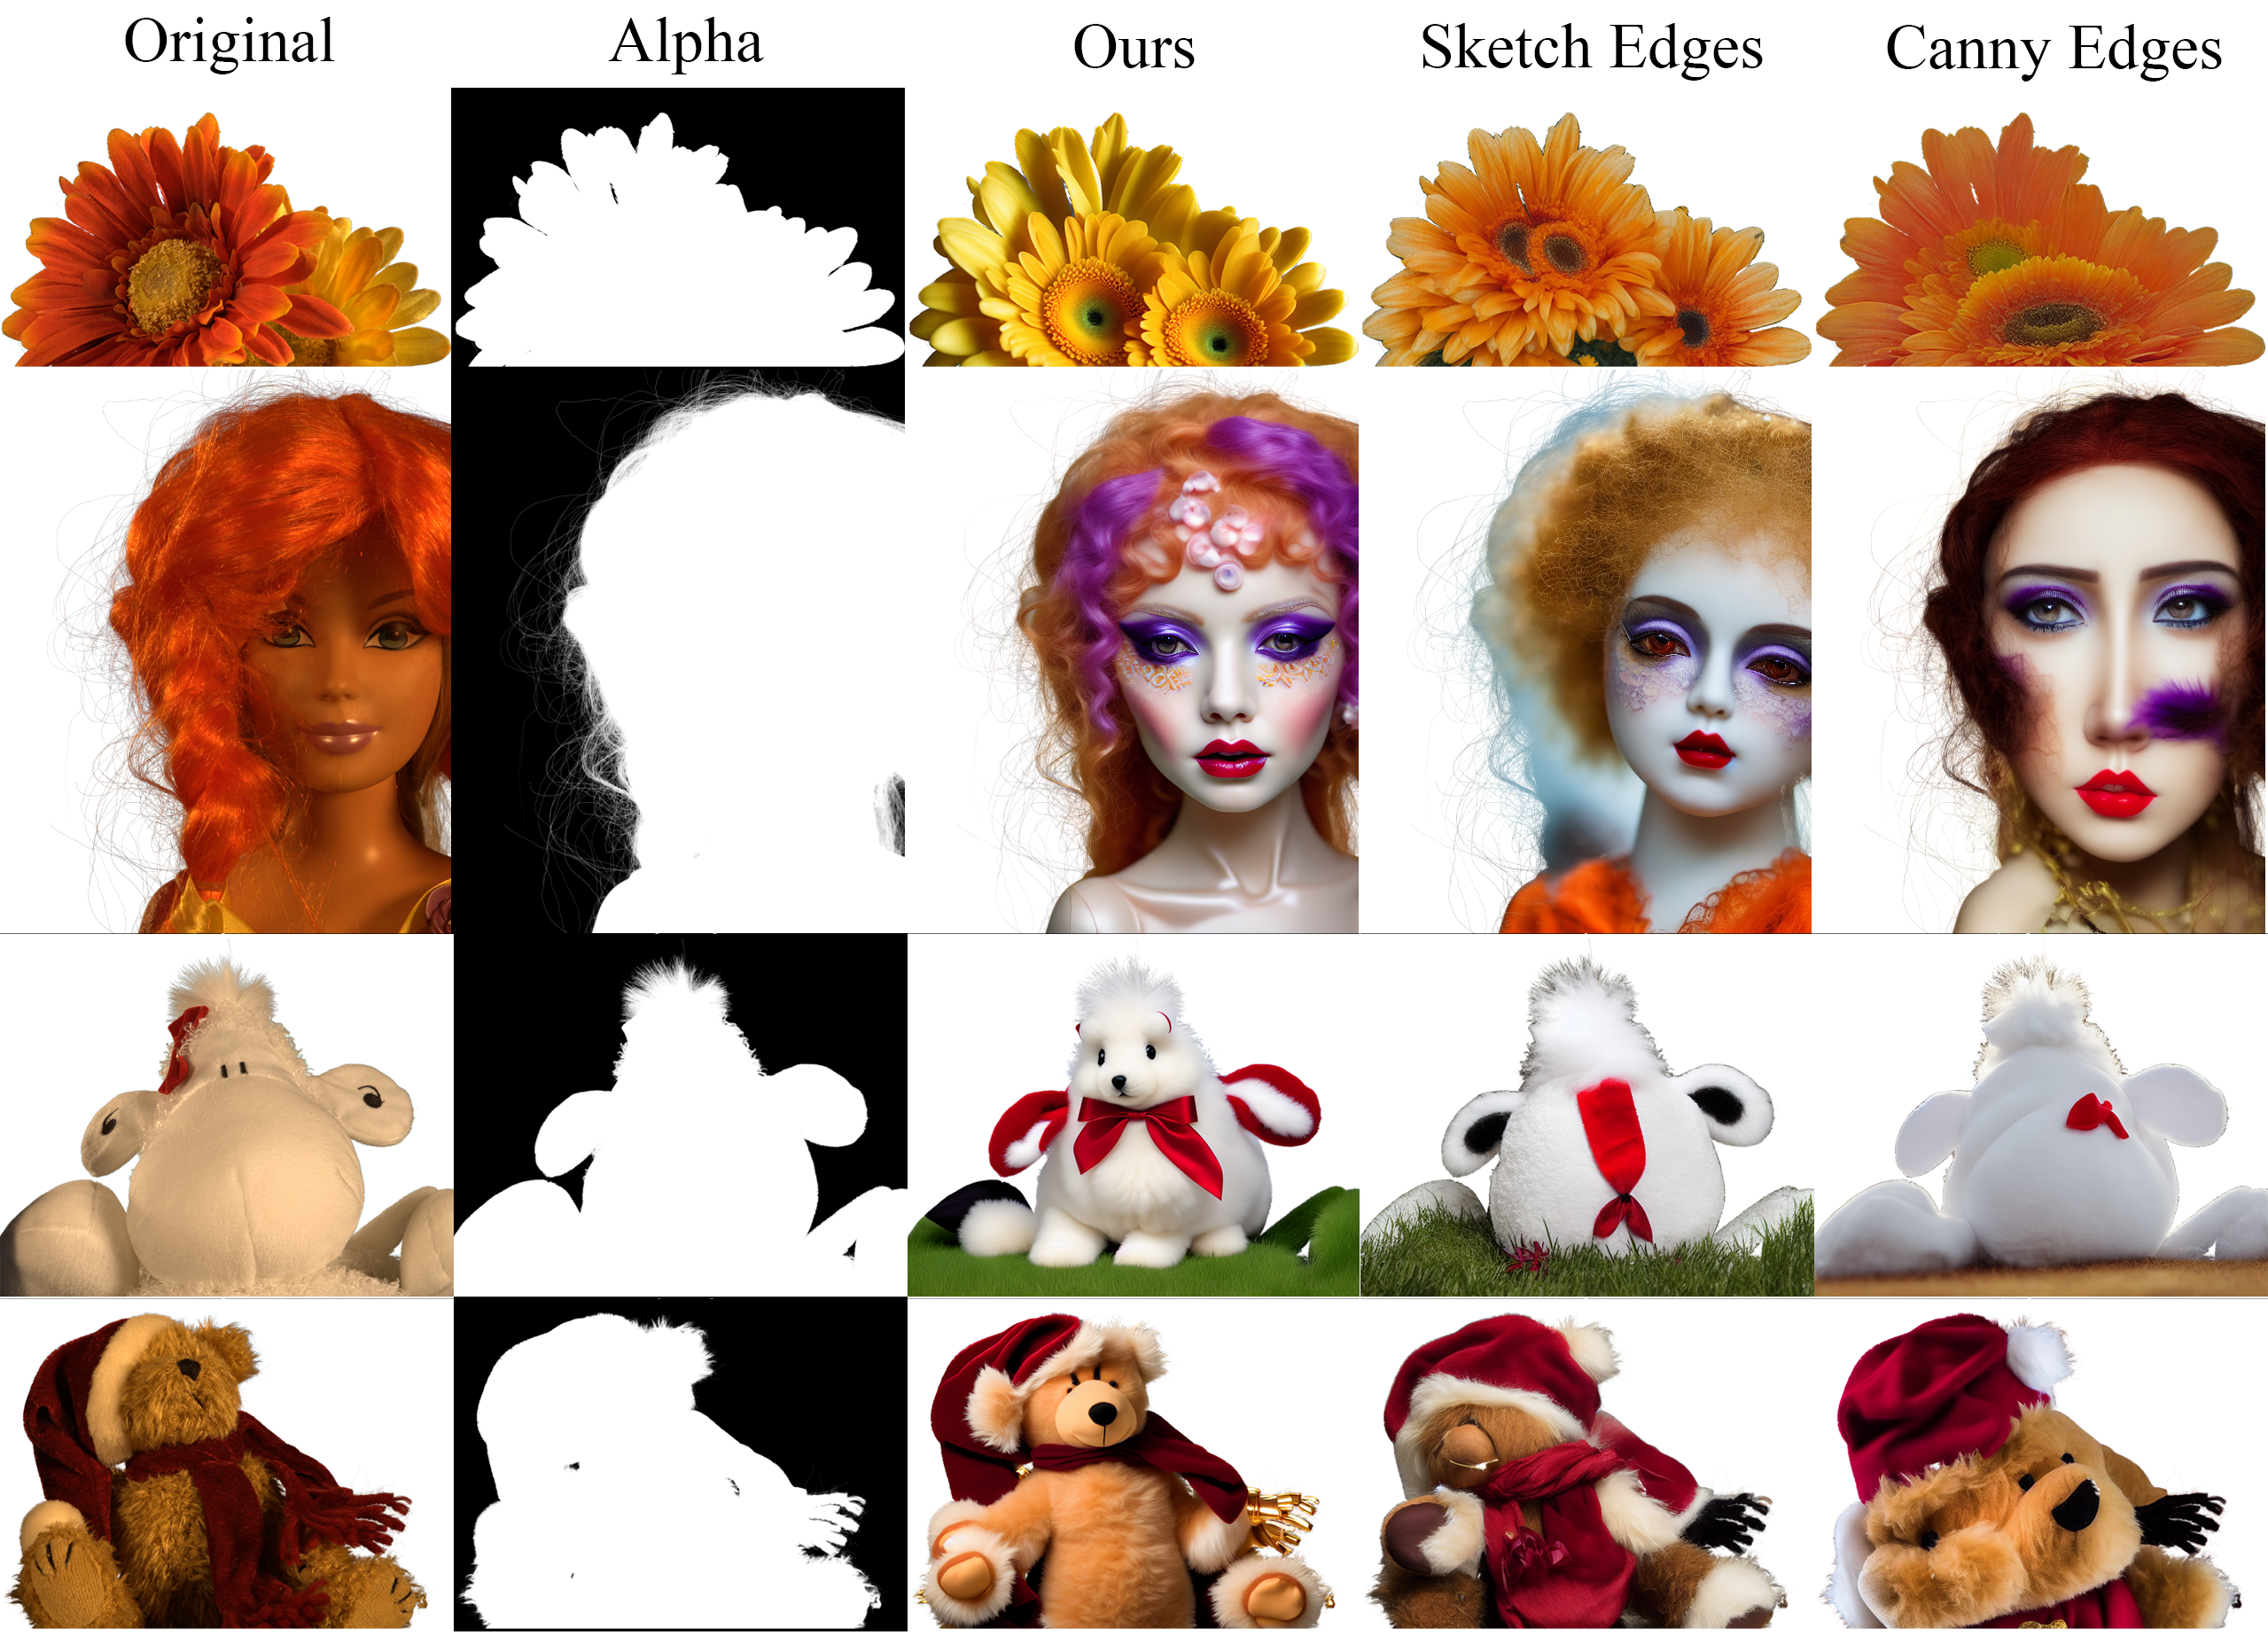
\includegraphics[width=1\linewidth]{figs/alpha2rgbResults.png}
    \vspace{-18pt}
    \caption{Generation results from our user study. The original images were the original images from~\cite{rhemann2009perceptually}, shown as reference and not used in the study. Given the alpha values and captions (not shown), images were generated using SD1.5 trained with our dataset, SD1.5 Sketch Edges, and SD1.5 Canny edges. }
    \label{fig:user_results}
\end{figure}



\begin{figure}
    \centering
    % 
\includegraphics[width=1\linewidth]{figs/S_s.png}
    \includegraphics[width=1\linewidth]{figs/S3.png}
    \vspace{-10pt}
    \caption{Example of alpha-to-rgb generation. The letter ``S'' is generated using different prompts to generate stylized text.}
    \label{fig:S}
\end{figure}




\begin{comment}
We trained ControlNet with SD1.5 on our dataset, to convert alpha mattes to RGB images. Because SD1.5 does RGB only, we generate images on perfect gray backgrounds. Given the orignal alpha matte an the generated image on gray, we can do math [insert alpha-blending inverse equation here] to recover the true colors.

We compare this against two baslines: canny edges controlet and scribble edges controlnet. These were both released with the original contronlet paper and both use SD1.5, making it a fair comparison because its the same algorithm and same base model. 

Our controlnet can take foreground masks and make images out of them. 

We had 52 users rate the images between ours and the baselines, and .82 of people prefer ours over canny edges controlnet and .77 prefer ours over scribblemaps. [TODO update numbers - they might be something like .03 different now]

The alpha mattes came from alphamatting.com, and the captions came from GPT4 after it was asked to caption the images. There are 27 images in total.
[TODO: add a figure showing some GPT4 captoins next to the original alphamatting.com images ]

[TODO: Get CLIP and LAION aesthetics scores for these imagees]

[TODO: Add a figure comparing ours qualitatively against text effects using all the images I put in the slack chat. might go in appendix though]

[TODO: add the illusion pictures. might go in appendix]

[TODO: Add some comparison RGBA images from LAION - they don't look as good. You can find them in one of the powerpoints - but that might also go inthe appendix.]
\end{comment}
\section{Conclusion}
\label{locvlm_sec:conclusion}

We introduce a simple framework that equips visual-LLMs (V-LLMs) with greater spatial understanding, termed LocVLM. We leverage the idea of encoding image coordinates within language to propose three instruction fine-tuning (IFT) objectives. This training process endows V-LLMs with the ability to reason about spatial composition of images using image space coordinates within text. A data efficient training pipeline utilizing pseudo-data allows our approach to achieve state-of-the-art results in Image VQA, Video VQA, and Region Description while improving spatial awareness and reducing object hallucination. 



{
    \small
    \bibliographystyle{ieeenat_fullname}
    \bibliography{main}
}




\clearpage
\setcounter{page}{1}


% \maketitlesupplementary %This messes up figure placement


\section{User Interface}

As a followup to \cref{sub:image_selection_process}, we discuss a specialized user interface we have developed for the manual annotation of this dataset, dramatically reducing the effort, time and cost of doing so.

Manual annotation, though less expensive than manual image matting (costing around \$30,000 and a few months), remains costly and time-consuming. To streamline this process, we've developed web-based program specifically for the task of selecting the best matte for subjects.

Along with the dataset, this tool will also be released to the public domain - in order to help people view and interact with this dataset before downloading it, as well as allowing people to easily expand it later on.

This tool simplifies the task by enabling annotators to quickly choose the best image from a set by simply clicking on it \cref{fig:ui}. Because it is web-based, it allows easy distribution of the annotation task: instead of having workers download the images to their local machines, terabytes of data can be streamed as they need it. Some key UI features include easy background color switching, alpha mask viewing with a single key-press, and workload distribution among multiple workers for parallel processing. 

Annotators are required to work with a dataset comprising RGBA images, which poses a challenge since there are no RGBA monitors — all physical pixels on a screen possess only RGB values. To circumvent this, we enable users to quickly view the alpha channel for samples and alternate the background color. This approach provides a clearer understanding of how the alpha mask influences the images.


% When the user's mouse is hovered over an image and the space bar is pressed, it zooms to full-screen. And when the letter `a' is pressed, it shows the alpha mask for that sample. This is better than zooming in manually to each sample, saving time and thus reducing the cost of annotation. There are many such quality of life features included like this.

This UI also includes search functionality as well, letting users search for images based on their captions. In \cref{fig:ui}, you can see that in the caption ``A crystal clear icicle hanging from a frozen branch'', the word ``icicle'' is bold and glowing - indicating the search term that matches that caption. There, the search term was ``icicle''. And in \cref{fig:tagging}, the search term ``letter'' was used.

Users can also tag images with tags such as ``\#nsfw,'' ``bad,'' and several other optional custom tags. Tags have many use cases, including: 
\begin{enumerate}
    \item It allows for the explicit annotation of poorly generated samples that lack good matting. Although this is a rare case, it still needs to be addressed.
    \item It enables the categorization of samples. For instance, the ``\#nsfw'' tag, represented as a button below the image samples, when activated for a given sample, marks that sample as not safe for work.
    \item It permits marking samples as ``\#idk'', which indicates that the sample requires review by another annotator. Since tags are searchable, if the user searches ``\#idk'', all samples marked as such will appear and can be reviewed.
\end{enumerate}


A live server for our dataset, along with the code and a user manual will be released for free to the public along with this paper. We hope by doing so we can encourage others to help grow the manually annotated portion of this dataset further.




\section{Additional Dataset Statistics}
Our data-set contains both safe-for-work and NSFW content, which is labeled as such. Approximately $.15\%$ of the samples in our dataset are flagged NSFW, as determined by a combination of the human annotators and a check for over 3000 blacklisted keywords present in the subjects. 

Additionally, the dataset contains a mix of shadows and non-shadows - as some samples will include soft shadows in their alpha-matte. 

The whole dataset generation process was accomplished on 32 A100 GPUs over the span of three weeks, plus an additional two months of human annotation with a budget of \$30000 USD. 

As mentioned in \cref{sub:least_common_hue},
green and blue are the most common hues in our dataset. The exact distribution is shown in \cref{fig:leastCommonHueDistribution}.
\begin{figure}
    %FOR BRIAN: This graph was generated with python code. To generate your own variant use the following link:
    %SOURCE: https://gist.github.com/SqrtRyan/bfb40468a3b52d0ca5ac5c20105f3ea2
    \centering
    % \includegraphics[width=1\linewidth]{figs/LeastCommonHueDistribution.png} %A taller version of the graph
    \includegraphics[width=1\linewidth]{figs/ShorterLeastCommonHueDistribution.png}
    \vspace{-20pt}
    \caption{Green backgrounds and blue backgrounds are by far the most common backgrounds used in our dataset, followed by magenta and rarely yellow or red. Green and blue are generally great colors for chroma keying, especially against human subjects.}
    \label{fig:leastCommonHueDistribution}
\end{figure}










\begin{figure*}  % Position specifiers added
    \centering
    \includegraphics[width=.9\textwidth]{figs/ui3.png}  % Adjusted the width to be less than \columnwidth
    \caption{A web-based annotation program designed specifically for the task of creating this dataset. Combinations of the alpha and foreground colors from three primary matting methods are shown in the columns. For each image, the user clicks the best one. In this example, the background color is set to red.}
    \label{fig:ui}
\end{figure*}

\begin{figure*}
    \centering
    \includegraphics[width=.9\linewidth]{figs/ui4.png}
    % \includegraphics[width=1\linewidth]{figs/tagging.png}
    \caption{An example of tagging the results. Here, we marked all images of the letter P as `review' - which lets us filter them out later.}
    \label{fig:tagging}
\end{figure*}









\section{User Study Details}
As mentioned in \cref{sec:application_alpha_to_rgb}, we provide all images used in our user study in this supplementary material, in \cref{fig:userstudy_full} - a continuation of \cref{fig:user_results}.


\section{Selecting Prompts (Continued)}
In \cref{sub:selecting_prompts} we listed three methods of generating prompts:
\begin{enumerate}
    \item LLM-Generated Prompts
    \item Procedurally Generated Prompts
    \item Image Captions
\end{enumerate}


In this section we will give examples for each category.


\subsection{LLM-Generated Prompts} 

What we send to GPT4:

\lstset{
    basicstyle=\promptExampleSize\ttfamily,
    breaklines=true,
    % postbreak=\mbox{\textcolor{red}{$\hookrightarrow$}\space},
}

\begin{lstlisting}
We are generating a large synthetic dataset of images with complex alpha mattes.
Please generate a list of image prompts with the following themes:
[water, fire, feathers, hair, glass, humans, animals] + any other themes with complex alpha mattes
DO NOT describe entire scenes, and DO NOT specify backgrounds - declare ONLY a single well-described isolated foreground subject.
The output format should be a code block with at least 500 line-separated prompts.
\end{lstlisting}

An example output from GPT4: 
\begin{enumerate}[noitemsep]
    %Shuffled Short Prompts:
    {\promptExampleSize \item \texttt{A lock of wavy, sunlit blonde hair.}}
    {\promptExampleSize \item \texttt{A frosted glass sculpture of a swan.}}
    {\promptExampleSize \item \texttt{A detailed macro shot of a butterfly wing.}}
    {\promptExampleSize \item \texttt{A swirling vortex of crystal-clear water.}}
    {\promptExampleSize \item \texttt{A swirling tornado of fire and ash.}}
    {\promptExampleSize \item \texttt{A soap bubble just before it bursts.}}
    {\promptExampleSize \item \texttt{A detailed close-up of a human iris.}}
    {\promptExampleSize \item \texttt{A single water droplet on a lotus leaf.}}
    {\promptExampleSize \item \texttt{A piece of amber glass reflecting sunlight.}}
    {\promptExampleSize \item \texttt{A single strand of barbed wire with dew drops.}}
    {\promptExampleSize \item \texttt{A bonfire with intense, twisting flames.}}
    {\promptExampleSize \item \texttt{A close-up of intricate lacework.}}
    {\promptExampleSize \item \texttt{A glowing ember in a dying fire.}}
    {\promptExampleSize \item \texttt{A close-up of a dragonfly's wing.}}
    {\promptExampleSize \item \texttt{A close-up of frost patterns on a window.}}
    {\promptExampleSize \item \texttt{A bubble reflecting a rainbow of colors.}}
    {\promptExampleSize \item \texttt{A eagle's feather with detailed texture.}}

\end{enumerate}


\subsection{Procedurally Generated Prompts}
\begin{enumerate}[noitemsep]
    {\promptExampleSize \item \texttt{anxious man big ears}}
    {\promptExampleSize \item \texttt{black escape artist man}}
    {\promptExampleSize \item \texttt{bored physician girl}}
    {\promptExampleSize \item \texttt{elderly personal care aide boy}}
    {\promptExampleSize \item \texttt{excited old psychic person}}
    {\promptExampleSize \item \texttt{firefighter woman closed eyes}}
    {\promptExampleSize \item \texttt{gay stablehand woman}}
    {\promptExampleSize \item \texttt{hispanic barista man with black flowing hair}}
    {\promptExampleSize \item \texttt{lawyer woman diamond earrings}}
    {\promptExampleSize \item \texttt{man wearing purple skirt}}
    {\promptExampleSize \item \texttt{necromancer man brown eyes}}
    {\promptExampleSize \item \texttt{nurse person green eyes}}
    {\promptExampleSize \item \texttt{person wearing gown}}
    {\promptExampleSize \item \texttt{sad fairy girl hazel eyes}}
    {\promptExampleSize \item \texttt{seamstress girl standing}}
    {\promptExampleSize \item \texttt{software engineer boy big ears}}
    {\promptExampleSize \item \texttt{teenage gay nurse man}}
    {\promptExampleSize \item \texttt{waiter man beard waving}}
    {\promptExampleSize \item \texttt{white boy with curly hair}}
    {\promptExampleSize \item \texttt{woman with red spiky hair}}
\end{enumerate}

\subsection{Image Captions}
\begin{enumerate}[noitemsep]
    {\promptExampleSize \item \texttt{Close-up of a new basketball ball}}
    {\promptExampleSize \item \texttt{Dairy products on a wooden table}}
    {\promptExampleSize \item \texttt{Deliciously refined tangerines}}
    {\promptExampleSize \item \texttt{Dog in a hat laborer looking at the camera}}
    {\promptExampleSize \item \texttt{Dried betel nuts or areca nuts}}
    {\promptExampleSize \item \texttt{Flying bird from black smooth lines}}
    {\promptExampleSize \item \texttt{Fresh artichokes close-up on dark background}}
    {\promptExampleSize \item \texttt{Fresh lemon with lemon essential oil}}
    {\promptExampleSize \item \texttt{Glasses of tasty Negroni cocktail}}
    {\promptExampleSize \item \texttt{Green bush or wall of shrubs}}
    {\promptExampleSize \item \texttt{Heart sticker with the flag of Tajikistan}}
    {\promptExampleSize \item \texttt{Intertwined white textile fibers}}
    {\promptExampleSize \item \texttt{Number 14 made of wooden blocks}}
    {\promptExampleSize \item \texttt{Piggy bank with a vernier caliper}}
    {\promptExampleSize \item \texttt{Shiba Inu dog in a birthday cap}}
    {\promptExampleSize \item \texttt{Skyscraper building in 3D render}}
    {\promptExampleSize \item \texttt{Varnished beige elegant shoes}}
    {\promptExampleSize \item \texttt{White and brown chicken wings}}
    {\promptExampleSize \item \texttt{White bread toast with honey}}
    {\promptExampleSize \item \texttt{Young smiling woman posing in a studio}}
\end{enumerate}



























\section{Matting Experiments}
% \heading{Reviewers N9yT, eZzn: } \question{Using MAGICK to train matting models.}
% \phantomsection %This might let the label work..
% \label{sec:matting} %This doesn't work - I don't think you can add a label to something that's not a figure or section can you? The current compilation results in ?? --- I'll try something
 We trained a matting model from Dai et al, CVPR 2023 [7] under default settings on various training sets - comprised of images from both the MAGICK dataset and the Deep Image Matting (DIM) dataset. The ratio of datasets used varied; for example, a 1/3 ratio means 1/3 of the training images were from MAGICK, and 2/3 from DIM. Our results are in \cref{fig:matting}.

We evaluated the models on the DIM test set using the standard metrics. Our findings showed that a combined dataset approach yielded better results than using either the MAGICK or DIM datasets alone. The optimal performance was achieved with a mixture where 1/5 of the data was from MAGICK and 4/5 from DIM. %\todo{Do we have to explain what each metric - aka MSE, SAD, Conn and Grad mean? It's in the other paper and it took a paragraph to explain it there. -- NO}

We conclude that the MAGICK dataset is indeed useful for image matting, even though it was primarily designed for image generation - resulting in a considerable domain difference between the two datasets.

\begin{figure}[ht]
\vspace{-1em}
    \centering
    \begin{minipage}{0.35\linewidth}
        \centering
        \includegraphics[width=\linewidth]{figs/Graph.pdf}
        % \label{fig:graph}
    \end{minipage}%
    \begin{minipage}{0.65\linewidth}
        \centering
        \resizebox{\linewidth}{!}{
        \begin{tabular}{|c|c|c|c|c|}
            \hline
            Ratio & \textbf{MSE} & \textbf{SAD} & \textbf{Conn} & \textbf{Grad} \\ \hline
            \textbf{0}   & .0277 & 65.49 & 78.03 & 44.54 \\ 
            \textbf{1/3} & .0146 & 37.59 & 38.76 & 24.49 \\
            \textbf{1/2} & .0162 & 39.38 & 34.54 & 24.95 \\
            \textbf{2/3} & .0107 & \textbf{33.03} & 32.78 & 19.27 \\
            \textbf{4/5} & \textbf{.0104} & 33.51 & \textbf{32.26} & \textbf{18.62} \\
            \textbf{1}   & .0113 & 36.27 & 36.00 & 24.39 \\ \hline
        \end{tabular}
        
        }
        % \label{fig:table}


        %I noticed text in figures is smaller than the main text. It's strange but do you think we can save space by putting more of the matting section into the matting figure's caption?
        %We don't have room to explain things twice. It's probably better to explain in the text. I'd consider putting all figures in one figure with no caption at all to save space. They can figure out what refers to what. This isn't ideal, but we're low on time and space.
        %Figs 2 and 3 should be combined. The two images in Fig 3 can be stacked and put next to the Fig 2 image.
        %Ok! Should we delete the caption for figure 1? 
        %For now, I'd have one line so we can still refer to fig 1 and fig 2. But do what makes sense to fit everything in.
        %I need to leave now. I can try taking a look in a couple hours.
        %Ok, thank you for the help! I'll try combining the figures - do you think any of the main text needs additional work (so as not to make reviewers angry etc - I know they can be finicky)
        %I've edited a bit. I'll read over it once more really quickly
        \vspace{10pt}
    \end{minipage}
    \vspace{-1.3em}
    \caption{Matting results using MAGICK.}  %Keep captions to one line.
    %Preliminary results on mattingtrained with varying proportions of the MAGICK and Adobe Image Matting  datasets demonstrated optimal performance with a mix where 1/5 of the data was from MAGICK, outperforming the baseline of just using the Adobe Image Matting dataset.}
    \label{fig:matting}
    % \caption{To evaluate the effectiveness of MAGICK as an image matting dataset, we performed preliminary tests, training a matting model \cite{dai2022boosting} using their default settings on multiple training image sets, comprising of both our dataset and the Adobe Image Matting dataset \cite{xu2017deep} in different proportions. As the ratio increases, we use more of the Adobe Image Matting dataset and as it decreases we use more of our MAGICK dataset. A ratio of 1/3 for example refers to the results of training on a dataset where 1/3 of the training images come from our MAGICK dataset, and 2/3 of the training images come from the Adobe Image Matting dataset. We tested our models using the same procedure outlined in \cite{dai2022boosting}, \todo{do we need to explain these metrics? It would take up space. Right now I'm just referring them to the paper.} We tested on the Adobe Image Matting test set. The results of this test: using a mix of both datasets outperformed both using our MAGICK dataset alone or the Adobe Image Matting dataset alone - with an optimal mix where 1/5 of the data comes from our MAGICK dataset and 4/5 comes from the Adobe Image Matting dataset. We would like to highlight the fact that this is impressive, as the MAGICK dataset is primarily intended for image generation - and there is a significant domain shift between the two datasets.}
\end{figure}


\begin{figure*}[h!]
    \centering
    \includegraphics[width=.6\linewidth]{figs/autoselex.jpg}
    \caption{
    \textbf{Automatic selection:} Randomly generated images with similarity scores increasing from left to right. The top 50\%, highlighted in green, are kept while the rest are discarded. Samples with high similarity almost always have accurate alpha mattes.
    }
    \label{fig:auto_selection}
\end{figure*}

\begin{figure}[h!]
    \centering
    \includegraphics[width=1\linewidth]{figs/BeforeAfterImg2Img-crop.pdf}
    \caption{
    \textbf{SDEdit's Effect:} 6 more examples continuing \cref{fig:beforeAfterImg2Img} in the main paper. Note the extra detail given by SDEdit.
    }
    \label{fig:sdedit_effect}
\end{figure}


% \begin{comment}
% \begin{figure}
%     \centering
%     \includegraphics[width=.5\linewidth]{figs/sdedit_ablation_continued.pdf}
%     \caption{Continuing from Fig. 7 in the main paper, here are 3 more examples showcasing the effect of SDEdit on DeepFloyd-generated images. \todo{Make this much larger - include like 20 examples, with the entire pipeline - all the way from DeepFloyd's raw output to SDEdit. OR, if we REALLY need the space and HAVE To delete a figure, this is the first to go - it's the least important. But let's try spacing etc first }}
%     \label{fig:pipeline-examples}
% \end{figure}

% \begin{figure}
%     \centering
% %     \includegraphics[width=1\linewidth]{figs/tillycompcocomp.jpg}  %FOUR ROWS
%     % \includegraphics[width=1\linewidth]{figs/tillo_halved.jpg}   %TWO ROWS
%     \includegraphics[width=1\linewidth]{figs/singlerowhighlightedoooo.jpg} %ONE ROW
%     \caption{\textbf{Automatic selection (left):} Randomly generated images with similarity scores increasing from left to right. The top 50\%, highlighted in green, are kept while the rest are discarded. Samples with high similarity almost always have accurate alpha mattes. %While this automatic selection process rarely returns an image with a bad matte, it tends to reject highly transparent images with glass or shadows - a job which we left to human annotators.
%     }
%     \label{fig:simscores}
% \end{figure}

% \end{comment}





















\begin{figure*}[tb]
  \centering
  \includegraphics[width=\textwidth,height=\textheight,keepaspectratio]{figs/userstudy_full.jpg}
  \caption{Continuing from \cref{fig:user_results}, here we present all of the images used in the user study. Our algorithm was compared against both baselines.}
  \label{fig:userstudy_full}
\end{figure*}








\section{Qualitative Alpha-to-RGB Results}
In this section, we showcase many examples of Alpha-to-RGB generation, as described in \cref{sec:application_alpha_to_rgb}. 

There are many artistic applications our dataset here, such as applying styles to text.

Here are the figures we've included in this section:
\begin{enumerate}
    \item Text Stylization, along with comparisons to baselines: See \cref{fig:magick_styles}% and \cref{fig:magick_styles_b} (it's split into two parts).
    \item Optical Illusions: See \cref{fig:illusions}.
    \item More variants of the letter S, continuing \cref{fig:S}: See \cref{fig:S100}.
    \item Other Results: See \cref{fig:swirly_chess}.
\end{enumerate}

\section{Creation Effort}
Our dataset is comprised of both automatically selected images and manually selected images.
%
The automated part, forming 110k out of MAGICK's 150k images, involves negligible human effort. This process, as described in the paper, uses 32 A100 GPUs for three weeks, incurring only computational costs.
%
For manual section, comprising 40,000 images, we hired 5 workers who each worked 112 hours at a rate of \$0.3 USD per sample. Four of these workers were annotators, and the fifth was in charge of quality control.
%
%In future work, we plan to expand this MAGICK dataset by using these human annotations to train a classifier to automatically select the images missed by our current similarity-score-based automatic selection method (see  \cref{fig:simscores}), allowing us to create a much larger dataset without requiring manual annotation.
Human anotation requires  only one mouse click per sample.
Future work could include training a classifier model to replace the annotators.

% \todo{Please read this newly-added part}
\section{Limitations} MAGICK's main strength is its size - comprising of 150k images. However, its main limitation is that it is synthetic - inheriting both strengths and weaknesses from current diffusion models. For example, a sample with the caption ``stop sign'' will have a good alpha matte, but might spell ``stop'' incorrectly, as SDXL struggles with text.



\section{Extended Dataset Preview}
In addition to \cref{fig:datasetExpose}, which showcased 100 samples, this section presents an additional 1300 randomly selected samples from our dataset in figures \cref{fig:dataset1of4}, \cref{fig:dataset2of4}, \cref{fig:dataset3of4}, and \cref{fig:dataset4of4}.

The 1400 matted images exhibited in this document surpass the size of the previously largest general-purpose matting dataset \cite{sun2021semantic}, which contained 726 objects. Furthermore, the 1400 samples illustrated in this document represent less than 1\% of the entire MAGICK dataset, encompassing 150,000 samples, each at double the resolution of any figure depicted here.

\begin{figure*}
    \centering
    \includegraphics[width=1\linewidth]{figs/100_s.pdf}
    \caption{\textbf{Text Stylization}: \textit{This image is very high resolution - please zoom in!} Continuing \cref{fig:S}, we take the alpha mask of the letter S (inverted here for visibility), and apply our Alpha-to-RGB algorithm from \cref{sec:application_alpha_to_rgb} to it using 100 different prompts. %Note how precisely the outlines match - and how the shape helps decide the structure of its inner contents.
    }
    \label{fig:S100}
\end{figure*}

\begin{figure*}
    \centering
    % 
\includegraphics[width=1\linewidth]{figs/illusions.pdf} % For some reason I can't explain, this figure crashes PDF readers on my iPhone - but not on my laptop. No idea why. But I'll replace it with a png.
    \includegraphics[width=1\linewidth]{figs/NonCrashyIllusions.png}
    \hspace{-40pt}
    \caption{\textbf{Optical Illusions}: Our Alpha-to-RGB algorithm from \cref{sec:application_alpha_to_rgb} can be used to generate striking optical illusions. In each image, we use two prompts: one for each region of the alpha mask. On the top image, we fill in the classic goblet illusion: we use the prompts ``man and woman staring at each other'' along with ``a brass goblet''. On the bottom right image, we use the prompts ``a mountain range with snow-capped mountains'' and ``a mountain range with snow-capped mountains behind a dense green forest''. The log cabins and skiers were added after the fact for decoration. And on the left, a photograph of new york city was cut out, and the remaining mask was given the prompt ``a medieval castle'' and flipped upside-down and composited back onto the image of the city. Please view them upside-down! }
    \label{fig:illusions}
\end{figure*}


\begin{figure*}
    \centering
    % \includegraphics[width=1\linewidth]{figs/magick_styles_a.jpg}
    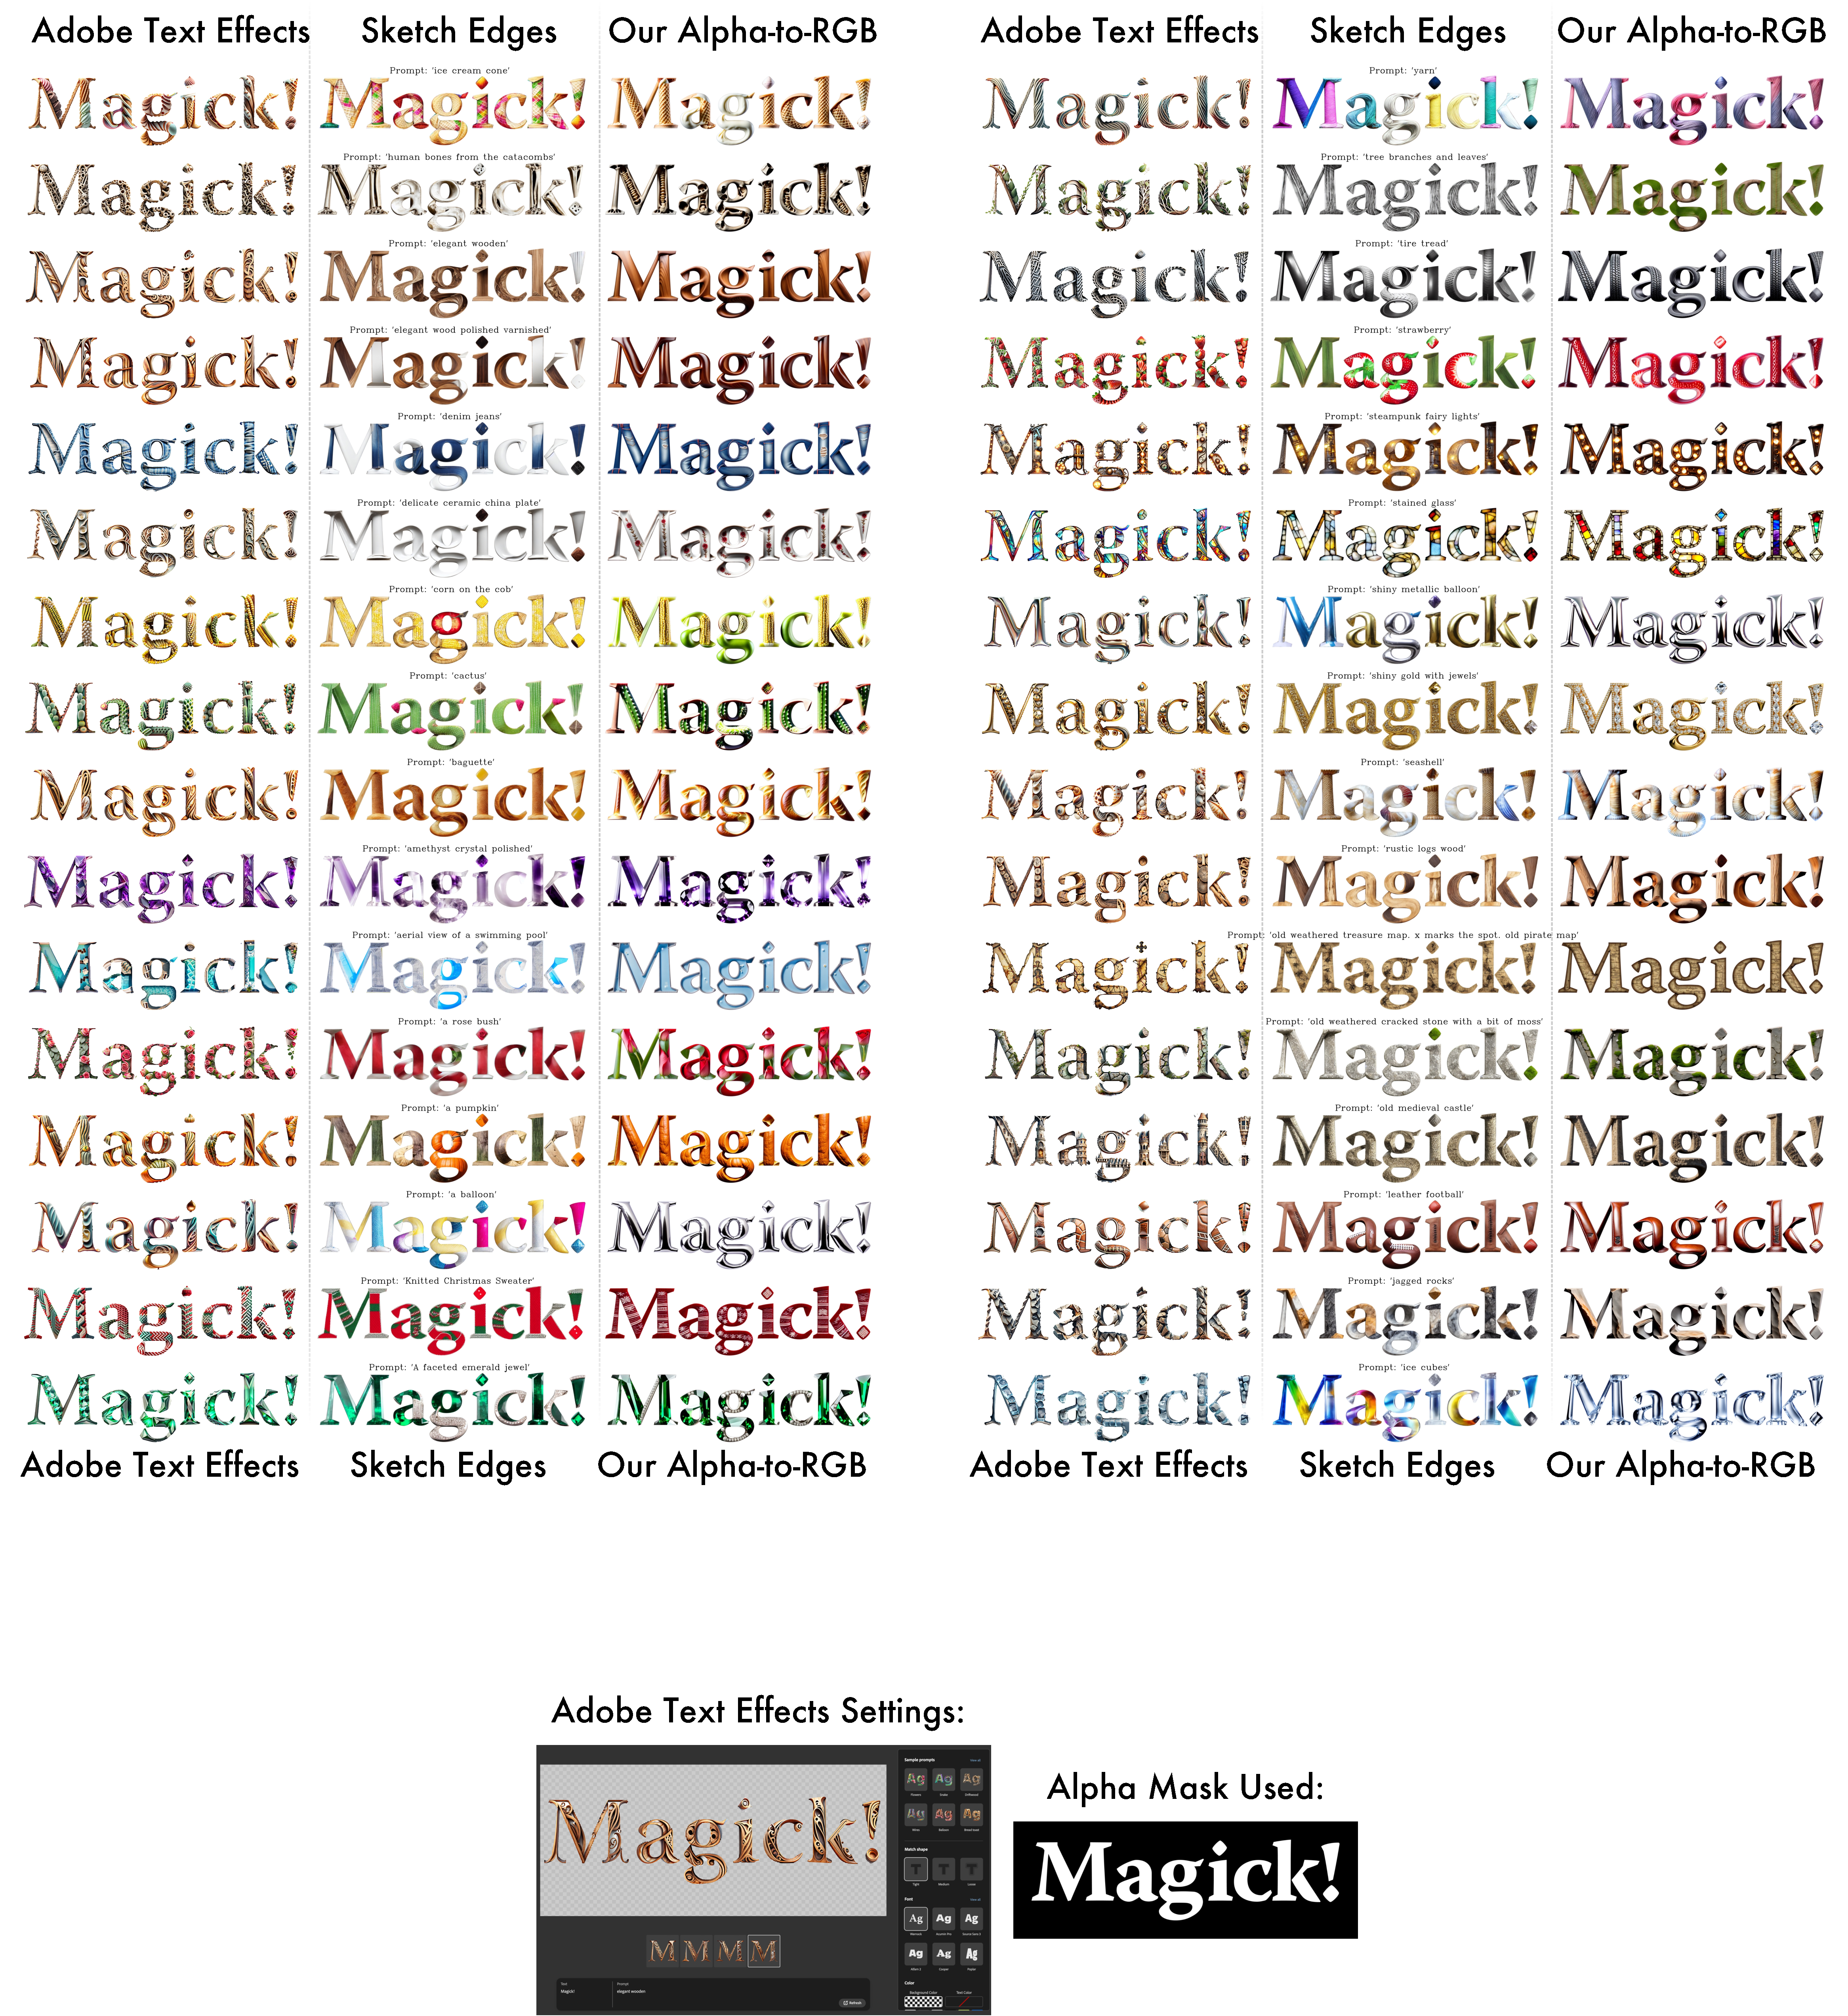
\includegraphics[width=1\linewidth]{figs/verymagick.pdf}
    \caption{\textbf{Text Stylization:} \textit{This image is very high resolution - please zoom in!} We apply our Alpha-to-RGB algorithm from \cref{sec:application_alpha_to_rgb} to the text ``Magick!'' in the font ``Warnock'', using many different styles. We compare it to two baselines: Adobe Text Effects and our Sketch Edges baseline from \cref{sec:application_alpha_to_rgb}. Note how the results from Adobe Text Effects don't always conform to the text boundary properly, despite the settings given to it (also depicted in this figure - its boundary mode is set to ``tight''). We chose to include the Sketch Edges baseline instead of the Canny Edges baseline because in our user study \cref{fig:user_results} it was the stronger-preferred of the two baselines.}
    \label{fig:magick_styles}
\end{figure*}


\begin{figure*}
    \centering
    \includegraphics[width=.7\linewidth]{figs/chess_swirl.jpg}
    \caption{Some more results of our Alpha-to-RGB algorithm \ref{sec:application_alpha_to_rgb}. The alpha masks are inverted for visibility.}
    \label{fig:swirly_chess}
\end{figure*}


\begin{figure*}
    \centering
    \includegraphics[width=1\linewidth]{ddpack0_q90.jpg}
    \caption{\textbf{Dataset Samples Part 1/4}: \textbf{Text Stylization:} \textit{This image is very high resolution - please zoom in!} This figure displays 325 random samples from our dataset, along with their alpha masks. Each sample also has a caption, not shown here.}
    \label{fig:dataset1of4}
\end{figure*}


\begin{figure*}
    \centering
    \includegraphics[width=1\linewidth]{figs/ddpack1_q90.jpg}
    \caption{\textbf{Dataset Samples Part 2/4}: \textbf{Text Stylization:} \textit{This image is very high resolution - please zoom in!} This figure displays 325 random samples from our dataset, along with their alpha masks. Each sample also has a caption, not shown here.}
    \label{fig:dataset2of4}
\end{figure*}

\begin{figure*}
    \centering
    \includegraphics[width=1\linewidth]{figs/ddpack2_q90.jpg}
    \caption{\textbf{Dataset Samples Part 3/4}: \textbf{Text Stylization:} \textit{This image is very high resolution - please zoom in!} This figure displays 325 random samples from our dataset, along with their alpha masks. Each sample also has a caption, not shown here.}
    \label{fig:dataset3of4}
\end{figure*}

\begin{figure*}
    \centering
    \includegraphics[width=1\linewidth]{figs/ddpack3_q90.jpg}
    \caption{\textbf{Dataset Samples Part 4/4}: \textbf{Text Stylization:} \textit{This image is very high resolution - please zoom in!} This figure displays 325 random samples from our dataset, along with their alpha masks. Each sample also has a caption, not shown here.}
    \label{fig:dataset4of4}
\end{figure*}


%%%%%%%%% REFERENCES


% \end{document}

% WARNING: do not forget to delete the supplementary pages from your submission 
% \clearpage
%\setcounter{page}{1}
\maketitlesupplementary

\section{Gaussianity preservation of our noise warping algorithm}

In this section, we discuss our noise warping algorithm, providing a formal proof of its Gaussianity preservation properties. We also present an illustrative example that demonstrates how noise that undergoes expansion and subsequent contraction returns to its original state, showcasing how our noise warping algorithm maintains the underlying Gaussian distribution throughout the warping process.

\begin{proof}
    For each $(x,y) \in V$, $R(x,y)$ is a collection of upsampled noise $X_i$, where
    \begin{align*}
    \bE[X_i] &= \bE[\frac{q(x,y)}{d}] + \bE[\frac{1}{\sqrt{d}}(Z_i - \frac{S}{d})] = 0  \\
        \Var(X_i) &= \Var(\frac{q(x,y)}{d}) + \Var(\frac{1}{\sqrt{d}}(Z_i - \frac{S}{d})) \\
        &= \frac{1}{d^2} + \frac{1}{d} \Var(\frac{d-1}{d}Z_i - \sum_{j\neq i} \frac{Z_j}{d}) \\
        &= \frac{1}{d^2} + \frac{1}{d} \frac{(d-1)^2 + (d-1)}{d^2} = \frac{1}{d},
    \end{align*}
    where we used the fact that $q(x,y)$ and $Z_i$'s are i.i.d. standard Gaussians.
    Since $X_i$ is constructed as a weighted sum of Gaussians, itself is also a Gaussian.
    Moreover, for $i \neq j$, we compute
    \begin{align*}
        &\Cov(X_i, X_j) \\
        =&\Cov(\frac{q(x,y)}{d} + \frac{1}{\sqrt{d}}(Z_i - \frac{S}{d}), \frac{q(x,y)}{d} + \frac{1}{\sqrt{d}}(Z_j - \frac{S}{d})) \\
        =& \frac{1}{d^2} + \frac{1}{d}\bE[(Z_i - \frac{S}{d})(Z_j - \frac{S}{d})] \\
        =& \frac{1}{d^2} + \frac{1}{d}(0 - 2 \frac{\bE[Z_i S]}{d} + \frac{\bE[S^2]}{d^2}) \\
        =& \frac{1}{d^2} + \frac{1}{d}(-\frac{2}{d} + \frac{1}{d}) = 0.
    \end{align*}
    Hence all $X_i$'s are independent.

    For each $(x',y') \in V'$, if $\deg_G((x',y')) = 0$, then $q'(x',y')$ is sampled as an independent standard Gaussian. 
    Otherwise, the output noise pixel $q'(x',y')$ is built as a weighted sum of $R(x,y)\text{.pop}()$ for each edge $((x,y), (x',y'))\in E$, where $R(x,y)\text{.pop}()$ is an independent Gaussian of mean 0 and variance $\frac{1}{\deg_G((x,y))}$.
    Hence $q'(x',y')$ is also a Gaussian with mean 0.
    The variable $s$ after executing the inner for loop thus represents the variance of $q'(x',y')$, so the renormalization at the end brings $q'(x',y')$ back to a standard Gaussian.
    Since the composing $X_i$'s are independent, the resulting noise $q'$ should also have an independent Gaussian in each pixel.
\end{proof}

\begin{example}[Exact recovery of \expansion-\contraction]
Consider the following evolution of noise across three frames with forward flows $f_{i\to j}$ going from frame $i$ to frame $j$ with $i + 1 = j$ (and backward flow if $i -1 = j$).
Suppose at frame $1$, a pixel $v \in D$ with density $1$ has noise $q$. Suppose further that $v'_a$ is a pixel at frame $2$ such that $f_{1\to 2}^{-1}(v'_a) = \{v\}$, and $v'_b \in D$ is the only pixel at frame $2$ such that $f_{1\to 2}^{-1}(v_b') = \varnothing$ and $f_{2\to 1}(v'_b) = v$.
This represents the scenario where $v$ is expanded into two pixels $v'_a,v'_b$.
Then \cref{alg:main} with forward flow $f_{1\to 2}$ and backward flow $f_{2 \to 1}$ will result in $v'_a$ having density $1/2$ and noise $\frac{q}{2} + \frac{1}{\sqrt{2}}(\frac{Z_a-Z_b}{2})$, and $v_b'$ having density $1/2$ and noise $\frac{q}{2} + \frac{1}{\sqrt{2}}(\frac{Z_b-Z_a}{2})$, where $Z_a$ and $Z_b$ are i.i.d. standard Gaussians.
Now, from frame $2$ to frame $3$, suppose there exists a pixel $v''$ such that $f_{2\to 3}^{-1}(v'') = \{v'_a,v'_b\}$, i.e., they both $v'_a$ and $v'_b$ contract to $v''$, and that $f_{3\to2}(D) \cap \{v'_a,v'_b\} = \varnothing$.
Then \cref{alg:main} with forward flow $f_{2\to 3}$ and backward flow $f_{3\to 2}$ will result in $v''$ having density $1$ and noise $q$, hence deterministically recovering the noise and density of $v$ in frame 0.

\end{example}


\section{Qualitative results of training-free image diffusion based video editing}

Noise warping methods that do not preserve Gaussianity degrade per-frame performance, as originally pointed out in~\cite{chang2024warped}. For example, using nearest neighbor and bilinear interpolation destroys the Gaussianity (see \cref{fig:supp_warped_noise_flow_vis}) and consequently deteriorates the per-frame performance on pre-trained image-to-image diffusion models (see \cref{fig:supp_davis_deepfloyd} and \cref{fig:supp_diffrelight_noisewarp}).

\begin{figure*}
    \centering
    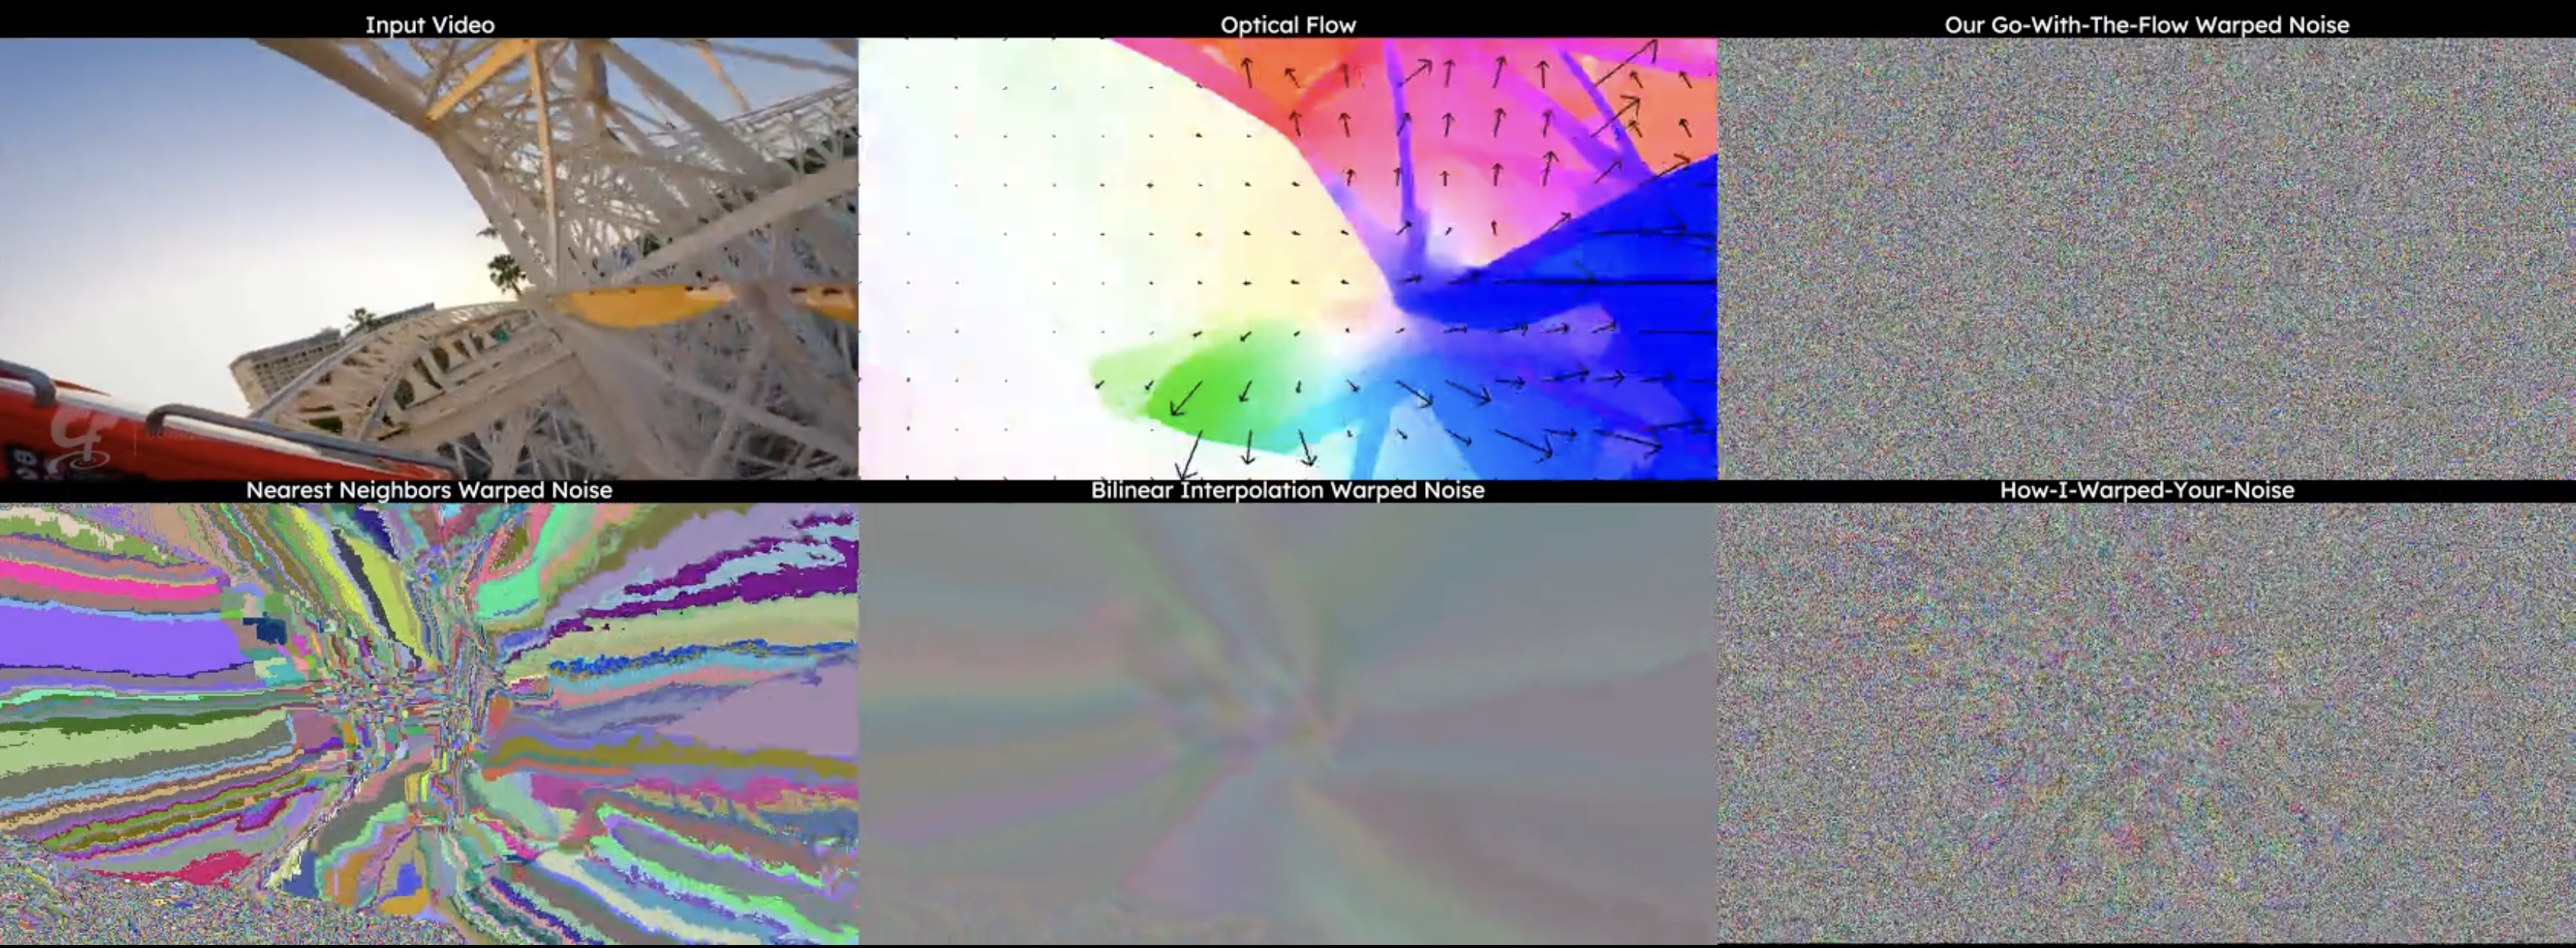
\includegraphics[width=1\linewidth]{fig/nongauss_vis.png}
    \caption{A direct visualization of the noise produced by our noise warping algorithm, HIWYN~\cite{chang2024warped}, bilinear, and nearest neighbor interpolations. The forward movement in this long roller-coaster video forces the noise to expand significantly. Early in the video, the HIWYN baseline produces visibly non-Gaussian results. See the full video on our \href{https://eyeline-research.github.io/Go-with-the-Flow/}{webpage}.}
    \label{fig:supp_warped_noise_flow_vis}
\end{figure*}

\begin{figure}
    \centering
    \includegraphics[width=1\linewidth]{fig/stroller_frame20.png}
    \caption{Using different noise warping algorithms on DeepFloyd~IF for video super-resolution on the DAVIS dataset.}
    \label{fig:supp_davis_deepfloyd}
\end{figure}

\begin{figure}
    \centering
    \includegraphics[width=1\linewidth]{fig/naz_diffrelight_grid11.jpg}
    \caption{Using different noise warping algorithms on DifFRelight for portrait video relighting. }
    \label{fig:supp_diffrelight_noisewarp}
\end{figure}


\section{The advantage of noise warping}

By using noise warping as a condition for motion, we effectively discard all structural information from our input video that cannot be inferred from motion alone. This can be advantageous, as demonstrated in \cref{fig:supp_windmill}. MotionClone does not use optical flow to guide the video trajectory, instead relying on manipulating activations within the diffusion model. As a result, the windmill gains an extra set of arms, whereas our method, which relies solely on motion information from optical flow via warped noise, does not introduce such artifacts.

\section{Comparison to the video diffusion base model without finetuning}

Interestingly, video diffusion models respond to noise warping even without training. In \cref{fig:supp_windmill} the rightmost column, even though the per-frame quality suffers, the flow of the output video still roughly follows the flow of the warped noise. However, because warped noise is statisically distinct from the pure Gaussian noise CogVideoX was trained on, without fine-tuning it can result in visual artifacts.

\section{User study settings and statistics}
\label{sec:supp_user_study}

\cref{fig:supp_user_study_screenshots_statistics} presents our user study questionnaires and statistics for two applications: (1) local object motion control, and (2) turnable camera movement video generation. Our questions focus on users' overall subjective preference, controllability, and temporal consistency.

\section{Model Agnostic}


Our method is data- and model-agnostic. It can be used to add motion control to arbitrary video diffusion models by only processing the noise sampling during fine-tuning. For example, it also works with AnimateDiff \cite{guo2024animatediff} fine-tuned on the WebVid dataset~\cite{Bain21} (the weights for this model on our \href{https://github.com/Eyeline-Research/Go-with-the-Flow}{GitHub} page). See its qualitative results in \cref{fig:supp_animatediff_grid}. Since release, the community has also trained a version of Go-with-the-Flow on HunyuanVideo (linked on our \href{https://github.com/Eyeline-Research/Go-with-the-Flow}{GitHub} page). Therefore, our method will generalize to future more advanced video diffusion base model.

\section{Pseudo code}

See \cref{listing:supp_algo_pseudo_code} for our noise warping pseudo code. See our source code and model checkpoints on \href{https://github.com/GoWithTheFlowPaper/gowiththeflowpaper.github.io}{GitHub}.

\begin{figure*}
    \centering
    \includegraphics[width=0.7\linewidth]{fig/windmills.pdf} 
    \caption{
    We show a \cutndrag~animation of a windmill rotating clockwise, next to the derived optical flow, our outputs, a baseline and an ablation. \textbf{Note} that the input video column appears to have two sets of panels because it's being cut and dragged over itself to create rotational motion. \textbf{When using noise warping is better}: Per-frame structural information can poison the result of MotionClone, giving the windmill an extra set of arms - whereas ours only receives motion information from optical flow alone via warped noise (there are no double-windmills in the optical flow patterns). \textbf{Ablation in rightmost column}: warped noise with $\deglevel=.5$ on the CogVideoX base model before we fine-tune it. Because warped noise is statisically distinct from the pure Gaussian noise CogVideoX was trained on, without fine-tuning it can result in visual artifacts. Note how although the per-frame quality suffers here, it still picks up on motion queues from the warped noise (the camera zooms into the windmill).}
    \label{fig:supp_windmill}
\end{figure*}

\begin{figure*}
    \centering
    \begin{subfigure}{.48\linewidth}
    \includegraphics[width=\linewidth]{fig/user_study_screenshot_1.png}
    \subcaption{User study interface and questions for local object motion control, corresponding to ~\cref{fig:comparisons_video_diffusion_object_motions} in the main paper.}
    \end{subfigure}
    \hfill
    \begin{subfigure}{.48\linewidth}
    \includegraphics[width=\linewidth]{fig/user_study_screenshot_2.png}
    \subcaption{User study interface and questions for turnable camera movement video generation, corresponding to ~\cref{fig:comparisons_video_diffusion_turning_object} in the main paper.}
    \end{subfigure}
    \\[12pt]
    \begin{subfigure}{0.48\linewidth}
    \centering
    \includegraphics[width=.7\linewidth]{fig/user_study_1_statistics_1.png}
    \subcaption{User study statistics for local object motion control on the first question ``\textit{Which video is the best overall?}''}
    \end{subfigure}
    \hfill
    \begin{subfigure}{0.48\linewidth}
    \centering
    \includegraphics[width=.7\linewidth]{fig/user_study_1_statistics_2.png}
    \subcaption{User study statistics for local object motion control on the second question ``\textit{Which video best aligns with the user intent for controlling the object movement based on the input?}''}
    \end{subfigure}
    \\[12pt]
    \begin{subfigure}{0.48\linewidth}
    \centering
    \includegraphics[width=.7\linewidth]{fig/user_study_1_statistics_1.png}
    \subcaption{User study statistics for local object motion control on the third question ``\textit{Which video best preserves the intended camera movement from the input?}''}
    \end{subfigure}
    \hfill
    \begin{subfigure}{0.48\linewidth}
    \centering
    \includegraphics[width=.7\linewidth]{fig/user_study_1_statistics_1.png}
    \subcaption{User study statistics for local object motion control on the fourth question ``\textit{Which video maintains the most consistent and stable motion throughout?}''}
    \end{subfigure}
    \\[12pt]
    \begin{subfigure}{0.48\linewidth}
    \centering
    \includegraphics[width=0.7\linewidth]{fig/user_study_2_statistics_1.png}
    \subcaption{User study statistics for motion transfer on the first question ``\textit{Which video has better overall quality?}''}
    \end{subfigure}
    \caption{User study questionnaires screenshots and statistics. For all the questions of both applications, our method (the rightmost bar plot) significantly wins the most user preferences.}
    \label{fig:supp_user_study_screenshots_statistics}
\end{figure*}

% \begin{figure*}
%     \centering
%     \includegraphics[width=1\linewidth]{fig/animatediff.jpg}
%     \caption{Fine-tuning AnimateDiff with our warped noise flow. All rows share the same movements, and all columns share the same text prompts. The first column is the reference video providing the flow to warp the noise in column 2, which is then used to diffuse all videos to the right. Please zoom in to see the captions for each row (input videos driving movement and warping noise via optical flow) and each column (text prompt for each video cell). Refer to our project video to see these in animation form.}
%     \label{fig:supp_animatediff_grid}
% \end{figure*}

\begin{figure*}
    \centering
    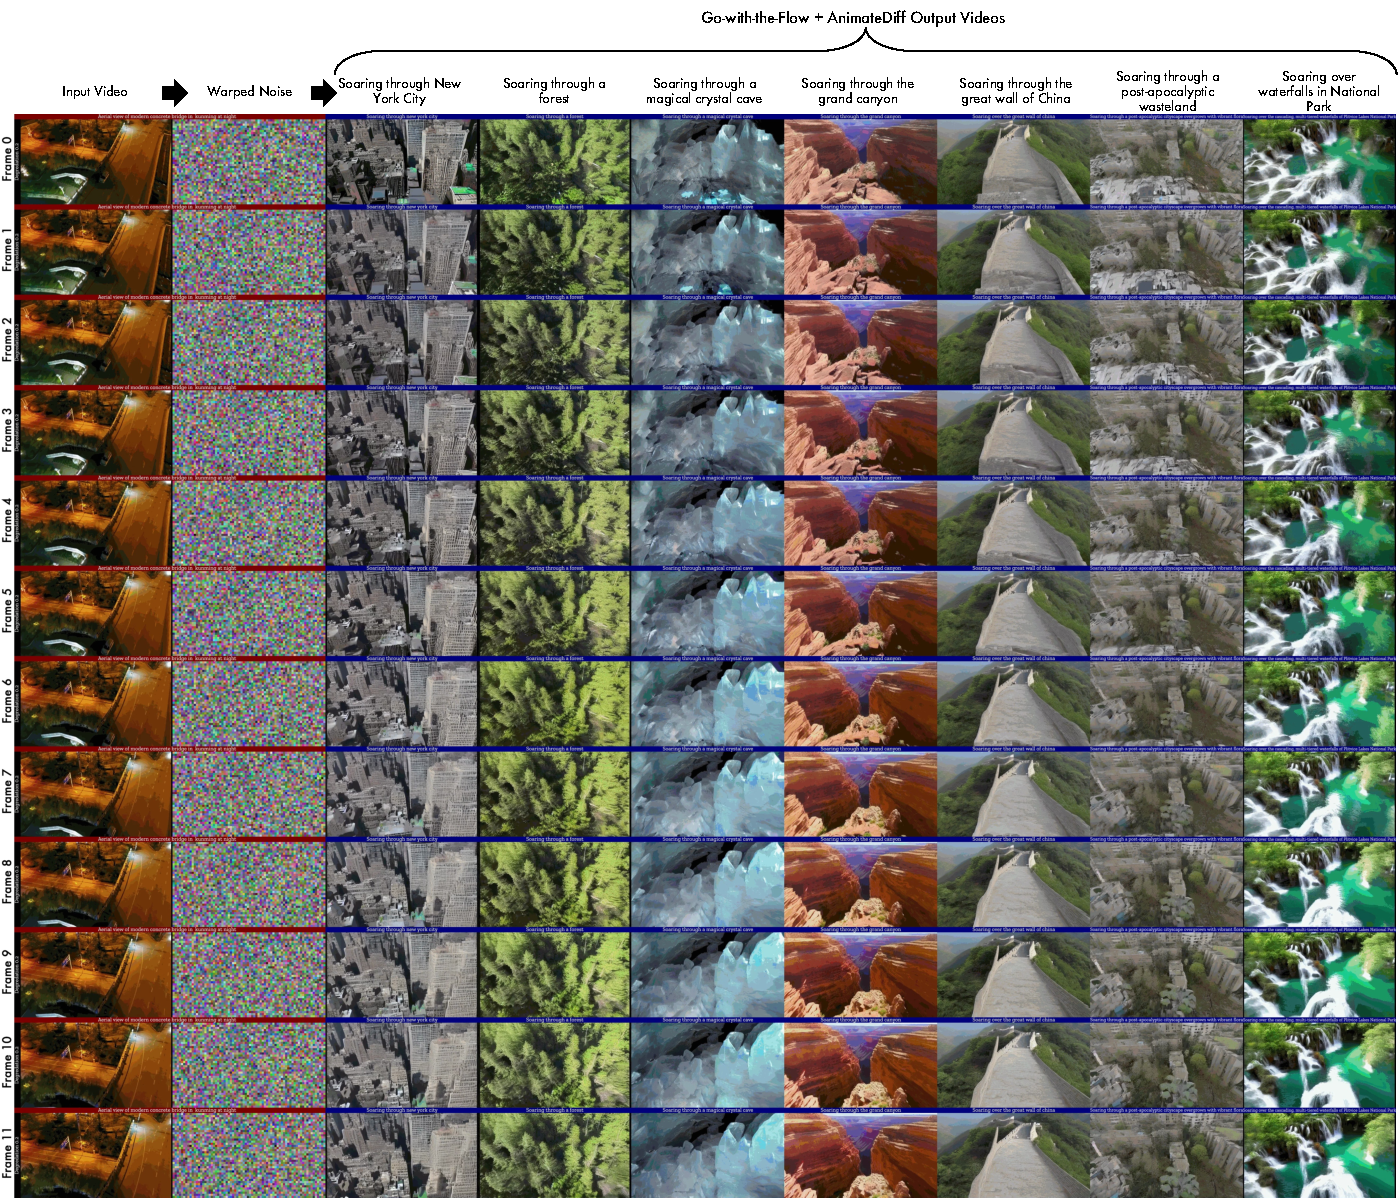
\includegraphics[width=1\linewidth]{fig/AnimateDiffAnimation.pdf}
    \caption{Fine-tuning AnimateDiff with our warped noise flow. We used Go-with-the-Flow to fine-tune AnimateDiff T2V, and display the results above. The input video is on the left, and from that video we derive warped noise which is used to initialize AnimateDiff on the columns to its right with different text prompts.}
    \label{fig:supp_animatediff_grid}
\end{figure*}

\begin{figure*}
\begin{lstlisting}
def warp_noise(prev_frame, cur_frame, prev_noise, prev_weight):

    height, width, _ = prev_frame.shape

    flow = optical_flow(prev_frame, cur_frame) # Agnostic to the optical flow algorithm
    backwards_flow = -flow # A cheap approximation of optical_flow(cur_frame, prev_frame)

    expansion_noise    = zeros(height, width)
    contraction_noise  = prev_noise.copy()

    expansion_mask     = ones (height, width, type=bool)
    contraction_mask   = zeros(height, width, type=bool)

    for x in range(width): for y in range(height):
        dx, dy = flow[x,y]
        if 0 <= x+dx <= width-1 and 0 <= y+dy <= height-1:
            # This particle stays in bounds
            expansion_mask  [x+dx, y+dx] = False
            contraction_mask[x   , y   ] = True  # Contraction mask is True where 

    for x in range(width): for y in range(height):
        if expansion_mask[x, y]:
            dx, dy = backwards_flow[x,y]
            expansion_noise [x, y] = prev_noise[x+dx, y+dy]

    # We've decided which source pixels are involved in contraction and expansion now
    contraction_noise &= contraction_mask
    expansion_noise, contraction_noise, cur_weight = jointly_regaussianize_and_rebalance_weights(
        expansion_noise, contraction_noise, prev_weight
    ) # Regaussianize all noise values here, and divide the weights by the number of pixels in each bin

    contraction_weight = zeros(height, width)
    for x in range(width): for y in range(height):
        if contraction_mask[x, y]:
            # Contraction treats the noise pixels as particles, each moving from the source to the
            # destination with this flow
            dx, dy = flow[x,y]
            # Contraction is a weighted sum of source pixels to a destination pixel
            pixel_weight = cur_weight[x, y]
            # Sum all the source noise pixels that contract to the same destination
            contraction_noise [x+dx, y+dy] += prev_noise[x, y] * pixel_weight
            # When we multiply a noise pixel by a weight, the variance changes by that weight squared
            contraction_weight[x+dx, y+dy] += pixel_weight ** 2 
    contraction_noise /= sqrt(contraction_weight) # Adjust the variance of the summed contracted noise

    # Mixing contraction and expansion noises with their respective masks
    cur_noise = contraction_noise & contraction_mask + expansion_noise & expansion_mask

    return cur_noise, cur_weight
\end{lstlisting}
\caption{Our noise warping pseudo code.}
\label{listing:supp_algo_pseudo_code}
\end{figure*}


% 


\clearpage
\setcounter{page}{1}


% \maketitlesupplementary %This messes up figure placement


\section{User Interface}

As a followup to \cref{sub:image_selection_process}, we discuss a specialized user interface we have developed for the manual annotation of this dataset, dramatically reducing the effort, time and cost of doing so.

Manual annotation, though less expensive than manual image matting (costing around \$30,000 and a few months), remains costly and time-consuming. To streamline this process, we've developed web-based program specifically for the task of selecting the best matte for subjects.

Along with the dataset, this tool will also be released to the public domain - in order to help people view and interact with this dataset before downloading it, as well as allowing people to easily expand it later on.

This tool simplifies the task by enabling annotators to quickly choose the best image from a set by simply clicking on it \cref{fig:ui}. Because it is web-based, it allows easy distribution of the annotation task: instead of having workers download the images to their local machines, terabytes of data can be streamed as they need it. Some key UI features include easy background color switching, alpha mask viewing with a single key-press, and workload distribution among multiple workers for parallel processing. 

Annotators are required to work with a dataset comprising RGBA images, which poses a challenge since there are no RGBA monitors — all physical pixels on a screen possess only RGB values. To circumvent this, we enable users to quickly view the alpha channel for samples and alternate the background color. This approach provides a clearer understanding of how the alpha mask influences the images.


% When the user's mouse is hovered over an image and the space bar is pressed, it zooms to full-screen. And when the letter `a' is pressed, it shows the alpha mask for that sample. This is better than zooming in manually to each sample, saving time and thus reducing the cost of annotation. There are many such quality of life features included like this.

This UI also includes search functionality as well, letting users search for images based on their captions. In \cref{fig:ui}, you can see that in the caption ``A crystal clear icicle hanging from a frozen branch'', the word ``icicle'' is bold and glowing - indicating the search term that matches that caption. There, the search term was ``icicle''. And in \cref{fig:tagging}, the search term ``letter'' was used.

Users can also tag images with tags such as ``\#nsfw,'' ``bad,'' and several other optional custom tags. Tags have many use cases, including: 
\begin{enumerate}
    \item It allows for the explicit annotation of poorly generated samples that lack good matting. Although this is a rare case, it still needs to be addressed.
    \item It enables the categorization of samples. For instance, the ``\#nsfw'' tag, represented as a button below the image samples, when activated for a given sample, marks that sample as not safe for work.
    \item It permits marking samples as ``\#idk'', which indicates that the sample requires review by another annotator. Since tags are searchable, if the user searches ``\#idk'', all samples marked as such will appear and can be reviewed.
\end{enumerate}


A live server for our dataset, along with the code and a user manual will be released for free to the public along with this paper. We hope by doing so we can encourage others to help grow the manually annotated portion of this dataset further.




\section{Additional Dataset Statistics}
Our data-set contains both safe-for-work and NSFW content, which is labeled as such. Approximately $.15\%$ of the samples in our dataset are flagged NSFW, as determined by a combination of the human annotators and a check for over 3000 blacklisted keywords present in the subjects. 

Additionally, the dataset contains a mix of shadows and non-shadows - as some samples will include soft shadows in their alpha-matte. 

The whole dataset generation process was accomplished on 32 A100 GPUs over the span of three weeks, plus an additional two months of human annotation with a budget of \$30000 USD. 

As mentioned in \cref{sub:least_common_hue},
green and blue are the most common hues in our dataset. The exact distribution is shown in \cref{fig:leastCommonHueDistribution}.
\begin{figure}
    %FOR BRIAN: This graph was generated with python code. To generate your own variant use the following link:
    %SOURCE: https://gist.github.com/SqrtRyan/bfb40468a3b52d0ca5ac5c20105f3ea2
    \centering
    % \includegraphics[width=1\linewidth]{figs/LeastCommonHueDistribution.png} %A taller version of the graph
    \includegraphics[width=1\linewidth]{figs/ShorterLeastCommonHueDistribution.png}
    \vspace{-20pt}
    \caption{Green backgrounds and blue backgrounds are by far the most common backgrounds used in our dataset, followed by magenta and rarely yellow or red. Green and blue are generally great colors for chroma keying, especially against human subjects.}
    \label{fig:leastCommonHueDistribution}
\end{figure}










\begin{figure*}  % Position specifiers added
    \centering
    \includegraphics[width=.9\textwidth]{figs/ui3.png}  % Adjusted the width to be less than \columnwidth
    \caption{A web-based annotation program designed specifically for the task of creating this dataset. Combinations of the alpha and foreground colors from three primary matting methods are shown in the columns. For each image, the user clicks the best one. In this example, the background color is set to red.}
    \label{fig:ui}
\end{figure*}

\begin{figure*}
    \centering
    \includegraphics[width=.9\linewidth]{figs/ui4.png}
    % \includegraphics[width=1\linewidth]{figs/tagging.png}
    \caption{An example of tagging the results. Here, we marked all images of the letter P as `review' - which lets us filter them out later.}
    \label{fig:tagging}
\end{figure*}









\section{User Study Details}
As mentioned in \cref{sec:application_alpha_to_rgb}, we provide all images used in our user study in this supplementary material, in \cref{fig:userstudy_full} - a continuation of \cref{fig:user_results}.


\section{Selecting Prompts (Continued)}
In \cref{sub:selecting_prompts} we listed three methods of generating prompts:
\begin{enumerate}
    \item LLM-Generated Prompts
    \item Procedurally Generated Prompts
    \item Image Captions
\end{enumerate}


In this section we will give examples for each category.


\subsection{LLM-Generated Prompts} 

What we send to GPT4:

\lstset{
    basicstyle=\promptExampleSize\ttfamily,
    breaklines=true,
    % postbreak=\mbox{\textcolor{red}{$\hookrightarrow$}\space},
}

\begin{lstlisting}
We are generating a large synthetic dataset of images with complex alpha mattes.
Please generate a list of image prompts with the following themes:
[water, fire, feathers, hair, glass, humans, animals] + any other themes with complex alpha mattes
DO NOT describe entire scenes, and DO NOT specify backgrounds - declare ONLY a single well-described isolated foreground subject.
The output format should be a code block with at least 500 line-separated prompts.
\end{lstlisting}

An example output from GPT4: 
\begin{enumerate}[noitemsep]
    %Shuffled Short Prompts:
    {\promptExampleSize \item \texttt{A lock of wavy, sunlit blonde hair.}}
    {\promptExampleSize \item \texttt{A frosted glass sculpture of a swan.}}
    {\promptExampleSize \item \texttt{A detailed macro shot of a butterfly wing.}}
    {\promptExampleSize \item \texttt{A swirling vortex of crystal-clear water.}}
    {\promptExampleSize \item \texttt{A swirling tornado of fire and ash.}}
    {\promptExampleSize \item \texttt{A soap bubble just before it bursts.}}
    {\promptExampleSize \item \texttt{A detailed close-up of a human iris.}}
    {\promptExampleSize \item \texttt{A single water droplet on a lotus leaf.}}
    {\promptExampleSize \item \texttt{A piece of amber glass reflecting sunlight.}}
    {\promptExampleSize \item \texttt{A single strand of barbed wire with dew drops.}}
    {\promptExampleSize \item \texttt{A bonfire with intense, twisting flames.}}
    {\promptExampleSize \item \texttt{A close-up of intricate lacework.}}
    {\promptExampleSize \item \texttt{A glowing ember in a dying fire.}}
    {\promptExampleSize \item \texttt{A close-up of a dragonfly's wing.}}
    {\promptExampleSize \item \texttt{A close-up of frost patterns on a window.}}
    {\promptExampleSize \item \texttt{A bubble reflecting a rainbow of colors.}}
    {\promptExampleSize \item \texttt{A eagle's feather with detailed texture.}}

\end{enumerate}


\subsection{Procedurally Generated Prompts}
\begin{enumerate}[noitemsep]
    {\promptExampleSize \item \texttt{anxious man big ears}}
    {\promptExampleSize \item \texttt{black escape artist man}}
    {\promptExampleSize \item \texttt{bored physician girl}}
    {\promptExampleSize \item \texttt{elderly personal care aide boy}}
    {\promptExampleSize \item \texttt{excited old psychic person}}
    {\promptExampleSize \item \texttt{firefighter woman closed eyes}}
    {\promptExampleSize \item \texttt{gay stablehand woman}}
    {\promptExampleSize \item \texttt{hispanic barista man with black flowing hair}}
    {\promptExampleSize \item \texttt{lawyer woman diamond earrings}}
    {\promptExampleSize \item \texttt{man wearing purple skirt}}
    {\promptExampleSize \item \texttt{necromancer man brown eyes}}
    {\promptExampleSize \item \texttt{nurse person green eyes}}
    {\promptExampleSize \item \texttt{person wearing gown}}
    {\promptExampleSize \item \texttt{sad fairy girl hazel eyes}}
    {\promptExampleSize \item \texttt{seamstress girl standing}}
    {\promptExampleSize \item \texttt{software engineer boy big ears}}
    {\promptExampleSize \item \texttt{teenage gay nurse man}}
    {\promptExampleSize \item \texttt{waiter man beard waving}}
    {\promptExampleSize \item \texttt{white boy with curly hair}}
    {\promptExampleSize \item \texttt{woman with red spiky hair}}
\end{enumerate}

\subsection{Image Captions}
\begin{enumerate}[noitemsep]
    {\promptExampleSize \item \texttt{Close-up of a new basketball ball}}
    {\promptExampleSize \item \texttt{Dairy products on a wooden table}}
    {\promptExampleSize \item \texttt{Deliciously refined tangerines}}
    {\promptExampleSize \item \texttt{Dog in a hat laborer looking at the camera}}
    {\promptExampleSize \item \texttt{Dried betel nuts or areca nuts}}
    {\promptExampleSize \item \texttt{Flying bird from black smooth lines}}
    {\promptExampleSize \item \texttt{Fresh artichokes close-up on dark background}}
    {\promptExampleSize \item \texttt{Fresh lemon with lemon essential oil}}
    {\promptExampleSize \item \texttt{Glasses of tasty Negroni cocktail}}
    {\promptExampleSize \item \texttt{Green bush or wall of shrubs}}
    {\promptExampleSize \item \texttt{Heart sticker with the flag of Tajikistan}}
    {\promptExampleSize \item \texttt{Intertwined white textile fibers}}
    {\promptExampleSize \item \texttt{Number 14 made of wooden blocks}}
    {\promptExampleSize \item \texttt{Piggy bank with a vernier caliper}}
    {\promptExampleSize \item \texttt{Shiba Inu dog in a birthday cap}}
    {\promptExampleSize \item \texttt{Skyscraper building in 3D render}}
    {\promptExampleSize \item \texttt{Varnished beige elegant shoes}}
    {\promptExampleSize \item \texttt{White and brown chicken wings}}
    {\promptExampleSize \item \texttt{White bread toast with honey}}
    {\promptExampleSize \item \texttt{Young smiling woman posing in a studio}}
\end{enumerate}



























\section{Matting Experiments}
% \heading{Reviewers N9yT, eZzn: } \question{Using MAGICK to train matting models.}
% \phantomsection %This might let the label work..
% \label{sec:matting} %This doesn't work - I don't think you can add a label to something that's not a figure or section can you? The current compilation results in ?? --- I'll try something
 We trained a matting model from Dai et al, CVPR 2023 [7] under default settings on various training sets - comprised of images from both the MAGICK dataset and the Deep Image Matting (DIM) dataset. The ratio of datasets used varied; for example, a 1/3 ratio means 1/3 of the training images were from MAGICK, and 2/3 from DIM. Our results are in \cref{fig:matting}.

We evaluated the models on the DIM test set using the standard metrics. Our findings showed that a combined dataset approach yielded better results than using either the MAGICK or DIM datasets alone. The optimal performance was achieved with a mixture where 1/5 of the data was from MAGICK and 4/5 from DIM. %\todo{Do we have to explain what each metric - aka MSE, SAD, Conn and Grad mean? It's in the other paper and it took a paragraph to explain it there. -- NO}

We conclude that the MAGICK dataset is indeed useful for image matting, even though it was primarily designed for image generation - resulting in a considerable domain difference between the two datasets.

\begin{figure}[ht]
\vspace{-1em}
    \centering
    \begin{minipage}{0.35\linewidth}
        \centering
        \includegraphics[width=\linewidth]{figs/Graph.pdf}
        % \label{fig:graph}
    \end{minipage}%
    \begin{minipage}{0.65\linewidth}
        \centering
        \resizebox{\linewidth}{!}{
        \begin{tabular}{|c|c|c|c|c|}
            \hline
            Ratio & \textbf{MSE} & \textbf{SAD} & \textbf{Conn} & \textbf{Grad} \\ \hline
            \textbf{0}   & .0277 & 65.49 & 78.03 & 44.54 \\ 
            \textbf{1/3} & .0146 & 37.59 & 38.76 & 24.49 \\
            \textbf{1/2} & .0162 & 39.38 & 34.54 & 24.95 \\
            \textbf{2/3} & .0107 & \textbf{33.03} & 32.78 & 19.27 \\
            \textbf{4/5} & \textbf{.0104} & 33.51 & \textbf{32.26} & \textbf{18.62} \\
            \textbf{1}   & .0113 & 36.27 & 36.00 & 24.39 \\ \hline
        \end{tabular}
        
        }
        % \label{fig:table}


        %I noticed text in figures is smaller than the main text. It's strange but do you think we can save space by putting more of the matting section into the matting figure's caption?
        %We don't have room to explain things twice. It's probably better to explain in the text. I'd consider putting all figures in one figure with no caption at all to save space. They can figure out what refers to what. This isn't ideal, but we're low on time and space.
        %Figs 2 and 3 should be combined. The two images in Fig 3 can be stacked and put next to the Fig 2 image.
        %Ok! Should we delete the caption for figure 1? 
        %For now, I'd have one line so we can still refer to fig 1 and fig 2. But do what makes sense to fit everything in.
        %I need to leave now. I can try taking a look in a couple hours.
        %Ok, thank you for the help! I'll try combining the figures - do you think any of the main text needs additional work (so as not to make reviewers angry etc - I know they can be finicky)
        %I've edited a bit. I'll read over it once more really quickly
        \vspace{10pt}
    \end{minipage}
    \vspace{-1.3em}
    \caption{Matting results using MAGICK.}  %Keep captions to one line.
    %Preliminary results on mattingtrained with varying proportions of the MAGICK and Adobe Image Matting  datasets demonstrated optimal performance with a mix where 1/5 of the data was from MAGICK, outperforming the baseline of just using the Adobe Image Matting dataset.}
    \label{fig:matting}
    % \caption{To evaluate the effectiveness of MAGICK as an image matting dataset, we performed preliminary tests, training a matting model \cite{dai2022boosting} using their default settings on multiple training image sets, comprising of both our dataset and the Adobe Image Matting dataset \cite{xu2017deep} in different proportions. As the ratio increases, we use more of the Adobe Image Matting dataset and as it decreases we use more of our MAGICK dataset. A ratio of 1/3 for example refers to the results of training on a dataset where 1/3 of the training images come from our MAGICK dataset, and 2/3 of the training images come from the Adobe Image Matting dataset. We tested our models using the same procedure outlined in \cite{dai2022boosting}, \todo{do we need to explain these metrics? It would take up space. Right now I'm just referring them to the paper.} We tested on the Adobe Image Matting test set. The results of this test: using a mix of both datasets outperformed both using our MAGICK dataset alone or the Adobe Image Matting dataset alone - with an optimal mix where 1/5 of the data comes from our MAGICK dataset and 4/5 comes from the Adobe Image Matting dataset. We would like to highlight the fact that this is impressive, as the MAGICK dataset is primarily intended for image generation - and there is a significant domain shift between the two datasets.}
\end{figure}


\begin{figure*}[h!]
    \centering
    \includegraphics[width=.6\linewidth]{figs/autoselex.jpg}
    \caption{
    \textbf{Automatic selection:} Randomly generated images with similarity scores increasing from left to right. The top 50\%, highlighted in green, are kept while the rest are discarded. Samples with high similarity almost always have accurate alpha mattes.
    }
    \label{fig:auto_selection}
\end{figure*}

\begin{figure}[h!]
    \centering
    \includegraphics[width=1\linewidth]{figs/BeforeAfterImg2Img-crop.pdf}
    \caption{
    \textbf{SDEdit's Effect:} 6 more examples continuing \cref{fig:beforeAfterImg2Img} in the main paper. Note the extra detail given by SDEdit.
    }
    \label{fig:sdedit_effect}
\end{figure}


% \begin{comment}
% \begin{figure}
%     \centering
%     \includegraphics[width=.5\linewidth]{figs/sdedit_ablation_continued.pdf}
%     \caption{Continuing from Fig. 7 in the main paper, here are 3 more examples showcasing the effect of SDEdit on DeepFloyd-generated images. \todo{Make this much larger - include like 20 examples, with the entire pipeline - all the way from DeepFloyd's raw output to SDEdit. OR, if we REALLY need the space and HAVE To delete a figure, this is the first to go - it's the least important. But let's try spacing etc first }}
%     \label{fig:pipeline-examples}
% \end{figure}

% \begin{figure}
%     \centering
% %     \includegraphics[width=1\linewidth]{figs/tillycompcocomp.jpg}  %FOUR ROWS
%     % \includegraphics[width=1\linewidth]{figs/tillo_halved.jpg}   %TWO ROWS
%     \includegraphics[width=1\linewidth]{figs/singlerowhighlightedoooo.jpg} %ONE ROW
%     \caption{\textbf{Automatic selection (left):} Randomly generated images with similarity scores increasing from left to right. The top 50\%, highlighted in green, are kept while the rest are discarded. Samples with high similarity almost always have accurate alpha mattes. %While this automatic selection process rarely returns an image with a bad matte, it tends to reject highly transparent images with glass or shadows - a job which we left to human annotators.
%     }
%     \label{fig:simscores}
% \end{figure}

% \end{comment}





















\begin{figure*}[tb]
  \centering
  \includegraphics[width=\textwidth,height=\textheight,keepaspectratio]{figs/userstudy_full.jpg}
  \caption{Continuing from \cref{fig:user_results}, here we present all of the images used in the user study. Our algorithm was compared against both baselines.}
  \label{fig:userstudy_full}
\end{figure*}








\section{Qualitative Alpha-to-RGB Results}
In this section, we showcase many examples of Alpha-to-RGB generation, as described in \cref{sec:application_alpha_to_rgb}. 

There are many artistic applications our dataset here, such as applying styles to text.

Here are the figures we've included in this section:
\begin{enumerate}
    \item Text Stylization, along with comparisons to baselines: See \cref{fig:magick_styles}% and \cref{fig:magick_styles_b} (it's split into two parts).
    \item Optical Illusions: See \cref{fig:illusions}.
    \item More variants of the letter S, continuing \cref{fig:S}: See \cref{fig:S100}.
    \item Other Results: See \cref{fig:swirly_chess}.
\end{enumerate}

\section{Creation Effort}
Our dataset is comprised of both automatically selected images and manually selected images.
%
The automated part, forming 110k out of MAGICK's 150k images, involves negligible human effort. This process, as described in the paper, uses 32 A100 GPUs for three weeks, incurring only computational costs.
%
For manual section, comprising 40,000 images, we hired 5 workers who each worked 112 hours at a rate of \$0.3 USD per sample. Four of these workers were annotators, and the fifth was in charge of quality control.
%
%In future work, we plan to expand this MAGICK dataset by using these human annotations to train a classifier to automatically select the images missed by our current similarity-score-based automatic selection method (see  \cref{fig:simscores}), allowing us to create a much larger dataset without requiring manual annotation.
Human anotation requires  only one mouse click per sample.
Future work could include training a classifier model to replace the annotators.

% \todo{Please read this newly-added part}
\section{Limitations} MAGICK's main strength is its size - comprising of 150k images. However, its main limitation is that it is synthetic - inheriting both strengths and weaknesses from current diffusion models. For example, a sample with the caption ``stop sign'' will have a good alpha matte, but might spell ``stop'' incorrectly, as SDXL struggles with text.



\section{Extended Dataset Preview}
In addition to \cref{fig:datasetExpose}, which showcased 100 samples, this section presents an additional 1300 randomly selected samples from our dataset in figures \cref{fig:dataset1of4}, \cref{fig:dataset2of4}, \cref{fig:dataset3of4}, and \cref{fig:dataset4of4}.

The 1400 matted images exhibited in this document surpass the size of the previously largest general-purpose matting dataset \cite{sun2021semantic}, which contained 726 objects. Furthermore, the 1400 samples illustrated in this document represent less than 1\% of the entire MAGICK dataset, encompassing 150,000 samples, each at double the resolution of any figure depicted here.

\begin{figure*}
    \centering
    \includegraphics[width=1\linewidth]{figs/100_s.pdf}
    \caption{\textbf{Text Stylization}: \textit{This image is very high resolution - please zoom in!} Continuing \cref{fig:S}, we take the alpha mask of the letter S (inverted here for visibility), and apply our Alpha-to-RGB algorithm from \cref{sec:application_alpha_to_rgb} to it using 100 different prompts. %Note how precisely the outlines match - and how the shape helps decide the structure of its inner contents.
    }
    \label{fig:S100}
\end{figure*}

\begin{figure*}
    \centering
    % \includegraphics[width=1\linewidth]{figs/illusions.pdf} % For some reason I can't explain, this figure crashes PDF readers on my iPhone - but not on my laptop. No idea why. But I'll replace it with a png.
    \includegraphics[width=1\linewidth]{figs/NonCrashyIllusions.png}
    \hspace{-40pt}
    \caption{\textbf{Optical Illusions}: Our Alpha-to-RGB algorithm from \cref{sec:application_alpha_to_rgb} can be used to generate striking optical illusions. In each image, we use two prompts: one for each region of the alpha mask. On the top image, we fill in the classic goblet illusion: we use the prompts ``man and woman staring at each other'' along with ``a brass goblet''. On the bottom right image, we use the prompts ``a mountain range with snow-capped mountains'' and ``a mountain range with snow-capped mountains behind a dense green forest''. The log cabins and skiers were added after the fact for decoration. And on the left, a photograph of new york city was cut out, and the remaining mask was given the prompt ``a medieval castle'' and flipped upside-down and composited back onto the image of the city. Please view them upside-down! }
    \label{fig:illusions}
\end{figure*}


\begin{figure*}
    \centering
    % \includegraphics[width=1\linewidth]{figs/magick_styles_a.jpg}
    \includegraphics[width=1\linewidth]{figs/verymagick.pdf}
    \caption{\textbf{Text Stylization:} \textit{This image is very high resolution - please zoom in!} We apply our Alpha-to-RGB algorithm from \cref{sec:application_alpha_to_rgb} to the text ``Magick!'' in the font ``Warnock'', using many different styles. We compare it to two baselines: Adobe Text Effects and our Sketch Edges baseline from \cref{sec:application_alpha_to_rgb}. Note how the results from Adobe Text Effects don't always conform to the text boundary properly, despite the settings given to it (also depicted in this figure - its boundary mode is set to ``tight''). We chose to include the Sketch Edges baseline instead of the Canny Edges baseline because in our user study \cref{fig:user_results} it was the stronger-preferred of the two baselines.}
    \label{fig:magick_styles}
\end{figure*}


\begin{figure*}
    \centering
    \includegraphics[width=.7\linewidth]{figs/chess_swirl.jpg}
    \caption{Some more results of our Alpha-to-RGB algorithm \ref{sec:application_alpha_to_rgb}. The alpha masks are inverted for visibility.}
    \label{fig:swirly_chess}
\end{figure*}


\begin{figure*}
    \centering
    \includegraphics[width=1\linewidth]{ddpack0_q90.jpg}
    \caption{\textbf{Dataset Samples Part 1/4}: \textbf{Text Stylization:} \textit{This image is very high resolution - please zoom in!} This figure displays 325 random samples from our dataset, along with their alpha masks. Each sample also has a caption, not shown here.}
    \label{fig:dataset1of4}
\end{figure*}


\begin{figure*}
    \centering
    \includegraphics[width=1\linewidth]{figs/ddpack1_q90.jpg}
    \caption{\textbf{Dataset Samples Part 2/4}: \textbf{Text Stylization:} \textit{This image is very high resolution - please zoom in!} This figure displays 325 random samples from our dataset, along with their alpha masks. Each sample also has a caption, not shown here.}
    \label{fig:dataset2of4}
\end{figure*}

\begin{figure*}
    \centering
    \includegraphics[width=1\linewidth]{figs/ddpack2_q90.jpg}
    \caption{\textbf{Dataset Samples Part 3/4}: \textbf{Text Stylization:} \textit{This image is very high resolution - please zoom in!} This figure displays 325 random samples from our dataset, along with their alpha masks. Each sample also has a caption, not shown here.}
    \label{fig:dataset3of4}
\end{figure*}

\begin{figure*}
    \centering
    \includegraphics[width=1\linewidth]{figs/ddpack3_q90.jpg}
    \caption{\textbf{Dataset Samples Part 4/4}: \textbf{Text Stylization:} \textit{This image is very high resolution - please zoom in!} This figure displays 325 random samples from our dataset, along with their alpha masks. Each sample also has a caption, not shown here.}
    \label{fig:dataset4of4}
\end{figure*}


%%%%%%%%% REFERENCES


% \end{document}


\end{document}
